%% USPSC-modelo-IQSC-DFQ.tex 
% ---------------------------------------------------------------
% USPSC: Modelo de Trabalho Academico (tese de doutorado, dissertacao de
% mestrado e trabalhos monograficos em geral) em conformidade com 
% ABNT NBR 14724:2011: Informacao e documentacao - Trabalhos academicos -
% Apresentacao
%----------------------------------------------------------------
%% Esta é uma customização do abntex2-modelo-trabalho-academico.tex de v-1.9.5 laurocesar 
%% para as Unidades do Campus USP de São Carlos:
%% EESC - Escola de Engenharia de São Carlos
%% IAU - Instituto de Arquitetura e Urbanismo
%% ICMC - Instituto de Ciências Matemáticas e de Computação
%% IFSC - Instituto de Física de São Carlos
%% IQSC - Instituto de Química de São Carlos
%%
%% Este trabalho utiliza a classe USPSC.cls que é mantida pela seguinte equipe:
%% 
%% Programação:
%%   - Marilza Aparecida Rodrigues Tognetti - marilza@sc.usp.br (PUSP-SC)
%%   - Ana Paula Aparecida Calabrez - aninha@sc.usp.br (PUSP-SC)
%% Normalização e Padronização:
%%   - Brianda de Oliveira Ordonho Sigolo - brianda@usp.br (IAU)
%%   - Elena Luzia Palloni Gonçalves - elena@sc.usp.br (EESC)
%%   - Eliana de Cássia Aquareli Cordeiro - eliana@iqsc.usp.br (IQSC)
%%   - Flávia Helena Cassin - cassinp@sc.usp.br (EESC)
%%   - Maria Cristina Cavarette Dziabas - mcdziaba@ifsc.usp.br (IFSC)
%%   - Regina Célia Vidal Medeiros - rcvmat@icmc.usp.br (ICMC)
%%
%% O USPSC-modelo.tex utiliza:	
%%  USPSC.cls e USPSC1.cls
%% 	USPSC-modelo-references.bib
%%	USPSC-modelo.tex
%%	USPSC-unidades.tex
%%	Um dos arquivos com dados pre-textuais abaixo, em conformidade com a Unidade de vínculo do autor:
%%				USPSC-pre-textual-EESC.tex
%%				USPSC-pre-textual-IAU.tex
%%				USPSC-pre-textual-ICMC.tex
%%				USPSC-pre-textual-IFSC.tex
%%				USPSC-pre-textual-IQSC.tex
%%				USPSC-pre-textual-OUTRO.tex
%%	USPSC-fichacatalografica.tex ou fichacatalografica.pdf
%%	folhadeaprovacao.pdf
%%	USPSC-Cap1-Introducao.tex
%%	USPSC-Cap2-Desenvolvimento.tex
%%	USPSC-Cap3-Citacoes.tex
%%	USPSC-Cap4-referencias.tex
%%	USPSC-Cap5-Conclusao.tex
%%	USPSC-Apendices.tex
%%	USPSC-Anexos.tex
%%	USPSC-AcentuacaoLaTeX.tex
%%	USPSC-LetrasGregas.tex
%%	USPSC-SimbolosUteis.tex

%----------------------------------------------------------------
%% Sobre a classe abntex2.cls:
%% abntex2.cls, v-1.9.5 laurocesar
%% Copyright 2012-2015 by abnTeX2 group at https://www.abntex.net.br/ 
%%
%----------------------------------------------------------------

\documentclass[
% -- opções da classe memoir --
12pt,		% tamanho da fonte
openright,	% capítulos começam em pág ímpar (insere página vazia caso preciso)
twoside,  % para impressão em anverso (frente) e verso. Oposto a oneside - Nota: utilizar \imprimirfolhaderosto*
%oneside, % para impressão em páginas separadas (somente anverso) -  Nota: utilizar \imprimirfolhaderosto
% inclua uma % antes do comando twoside e exclua a % antes do oneside 
a4paper,			% tamanho do papel. 
% -- opções da classe abntex2 --
chapter=TITLE,		% títulos de capítulos convertidos em letras maiúsculas
% -- opções do pacote babel --
english,			% idioma adicional para hifenização
french,				% idioma adicional para hifenização
spanish,			% idioma adicional para hifenização
brazil				% o último idioma é o principal do documento
% {USPSC} configura o cabeçalho contendo apenas o número da página
]{USPSC}
%]{USPSC1}
% Inclua % antes de ]{USPSC} e retire a % antes de %]{USPSC1}
% para utilizar o cabeçalho diferenciado para as páginas pares e ímpares como indicado abaixo:
%- páginas ímpares: cabeçalho com seções ou subseções e o número da página
%- páginas pares: cabeçalho com o número da página e o título do capítulo 
% ---

% ---
% Pacotes básicos - Fundamentais 
% ---
\usepackage[T1]{fontenc}		% Seleção de códigos de fonte.
\usepackage[utf8]{inputenc}		% Codificação do documento (conversão automática dos acentos)
\usepackage{lmodern}			% Usa a fonte Latin Modern
% Para utilizar a fonte Times New Roman, inclua uma % no início do comando acima  "\usepackage{lmodern}"
% Abaixo, tire a % antes do comando  \usepackage{times}
%\usepackage{times}		    	% Usa a fonte Times New Roman	
% Lembre-se de alterar a fonte no comando que imprime o preâmbulo no arquivo da Classe USPSC.cls				
\usepackage{lastpage}			% Usado pela Ficha catalográfica
\usepackage{indentfirst}		% Indenta o primeiro parágrafo de cada seção.
\usepackage{color}				% Controle das cores
\usepackage{graphicx}			% Inclusão de gráficos
\usepackage{float} 				% Fixa tabelas e figuras no local exato
\usepackage{chemfig,chemmacros} % Para escrever reações químicas
\usepackage{microtype} 			% para melhorias de justificação
\usepackage{pdfpages}
\usepackage{makeidx}            % para gerar índice remissimo
% ---

% ---
% Pacotes de citações
% Citações padrão ABNT
% ---
% Sistemas de chamada: autor-data ou numérico.
% Sistema autor-data
%\usepackage[alf,abnt-emphasize=bf, abnt-thesis-year=both, abnt-repeated-author-omit=yes, abnt-last-names=abnt, abnt-etal-cite,abnt-etal-list=3, abnt-etal-text=default, abnt-and-type=e, abnt-doi=doi, abnt-url-package=none, abnt-verbatim-entry=no]{abntex2cite}

% Para o IQSC, que indica todos os autores nas referências, incluir % no início do comando acima e retirar a % do comando abaixo 

\usepackage[alf,abnt-emphasize=bf, abnt-thesis-year=both, abnt-repeated-author-omit=yes, abnt-last-names=abnt, abnt-etal-cite,abnt-etal-list=0, abnt-etal-text=default, abnt-and-type=e]{abntex2cite}

% Sistema Numérico
% Para citações numéricas, sistema adotado pelo IFSC, incluir % no início do comando acima e retirar a % do comando abaixo 
%\usepackage[num,overcite,abnt-emphasize=bf, abnt-thesis-year=both, abnt-repeated-author-omit=yes, abnt-last-names=abnt, abnt-etal-cite,abnt-etal-list=0, abnt-etal-text=default, abnt-and-type=e]{abntex2cite}

% Complementarmente, verifique as instruções abaixo sobre os Pacotes de Nota de rodapé
% ---
% Pacotes de Nota de rodapé
% Configurações de nota de rodapé

% O presente modelo adota o formato numérico para as notas de rodapés quando utiliza o sistema de chamada autor-data para citações e referências. Para utilizar o sistema de chamada numérico para citações e referências, habilitar um dos comandos abaixo.
% Há diversa opções para nota de rodapé no Sistema Numérico.  Para o IFSC, habilitade o comando abaixo.

%\renewcommand{\thefootnote}{\fnsymbol{footnote}}  %Comando para inserção de símbolos em nota de rodapé

% Outras opções para nota de rodapé no Sistema Numérico:
%\renewcommand{\thefootnote}{\alph{footnote}}      %Comando para inserção de letras minúscula em nota de rodapé
%\renewcommand{\thefootnote}{\Alph{footnote}}      %Comando para inserção de letras maiúscula em nota de rodapé
%\renewcommand{\thefootnote}{\roman{footnote}}     %Comando para inserção de números romanos minúsculos  em nota de rodapé
%\renewcommand{\thefootnote}{\Roman{footnote}}     %Comando para inserção de números romanos minúsculos  em nota de rodapé

\renewcommand{\footnotesize}{\small} %Comando para diminuir a fonte das notas de rodapé

 % ---
 % Pacote para agrupar a citação numérica consecutiva
 % Quando for adotado o Sistema Numérico, a exemplo do IFSC, habilite 
 % o pacote cite abaixo retirando a porcentagem antes do comando abaixo
 %\usepackage[superscript]{cite}	

% ---
% Pacotes adicionais, usados apenas no âmbito do Modelo Canônico do abnteX2
% ---
\usepackage{lipsum}				% para geração de dummy text
% ---




% pacotes de tabelas
\usepackage{multicol}	% Suporte a mesclagens em colunas
\usepackage{multirow}	% Suporte a mesclagens em linhas
\usepackage{longtable}	% Tabelas com várias páginas
\usepackage{threeparttablex}    % notas no longtable
\usepackage{array}

%---
% Configurações para o pacote chemfig
%\chemsetup[chemformula]{format=\sffamily}
\renewcommand*\printatom[1]{\ensuremath{\mathsf{#1}}}
\setatomsep{2em}
\setdoublesep{.6ex}
\setbondstyle{semithick}
%---
% Configurando o ambiente para utilizar os recursos de frases pre-prontas do mhchem
\newenvironment{rslist}%
{%
	\begin{labeling}% environment from KOMA-script
		{\rsnumber{R39/23/24/25}}% R39/23/24/25 is longest label
	}{%
\end{labeling}%
}%
% Definição de comando para utilizar os recursos de frases pre-prontas do mhchem
\newcommand{\rs}[2][]{\item[{\rsnumber[#1]{#2}}] \rsphrase{bb}}
% ---

% ---
% DADOS INICIAIS - Define sigla com título, área de concentração e opção do Programa 
% Consulte a tabela referente aos Programas, áreas e opções de sua unidade contante do
% arquivo USPSC-Siglas estabelecidas para os Programas de Pós-Graduação por Unidade.xlsx 
% ou nos APÊNDICES A-G
\siglaunidade{IQSC} 
\programa{DFQ}
% Os demais dados deverão ser fornecidos no arquivo USPSC-pre-textual-UUUU ou USPSC-TCC-pre-textual-UUUU, onde UUUU é a sigla da Unidade. 
% Exemplo:USPSC-pre-textual-IFSC.tex
% ---
% Configurações de aparência do PDF final
% alterando o aspecto da cor azul
\definecolor{blue}{RGB}{41,5,195}

% informações do PDF
\makeatletter
\hypersetup{
	%pagebackref=true,
	pdftitle={\@title}, 
	pdfauthor={\@author},
	pdfsubject={\imprimirpreambulo},
	pdfcreator={LaTeX with abnTeX2},
	pdfkeywords={abnt}{latex}{abntex}{USPSC}{trabalho acadêmico}, 
	colorlinks=true,       		% false: boxed links; true: colored links
	linkcolor=blue,          	% color of internal links
	citecolor=blue,        		% color of links to bibliography
	filecolor=magenta,      		% color of file links
	urlcolor=blue,
	bookmarksdepth=4
}
\makeatother
% --- 
% --- 
% Espaçamentos entre linhas e parágrafos 
% --- 

% O tamanho do parágrafo é dado por:
\setlength{\parindent}{1.3cm}

% Controle do espaçamento entre um parágrafo e outro:
\setlength{\parskip}{0.2cm}  % tente também \onelineskip

% ---
% compila o sumário e índice
\makeindex
% ---

% ----
% Início do documento
% ----
\begin{document}

% Seleciona o idioma do documento (conforme pacotes do babel)
\selectlanguage{brazil}
% Se o idioma do texto for inglês, inclua uma % antes do 
%      comando \selectlanguage{brazil} e 
%      retire a % antes do comando abaixo
%\selectlanguage{english}

% Retira espaço extra obsoleto entre as frases.
\frenchspacing 

% --- Formatação dos Títulos
\renewcommand{\ABNTEXchapterfontsize}{\fontsize{12}{12}\bfseries}
\renewcommand{\ABNTEXsectionfontsize}{\fontsize{12}{12}\bfseries}
\renewcommand{\ABNTEXsubsectionfontsize}{\fontsize{12}{12}\normalfont}
\renewcommand{\ABNTEXsubsubsectionfontsize}{\fontsize{12}{12}\normalfont}
\renewcommand{\ABNTEXsubsubsubsectionfontsize}{\fontsize{12}{12}\normalfont}


% ----------------------------------------------------------
% ELEMENTOS PRÉ-TEXTUAIS
% ----------------------------------------------------------
% ---
% Capa
% ---
\imprimircapa
% ---
% Folha de rosto
% (o * indica impressão em anverso (frente) e verso )
% ---
\imprimirfolhaderosto*
%\imprimirfolhaderosto
% ---
% ---
% Inserir a ficha catalográfica em pdf
% ---
% A biblioteca da sua Unidade lhe fornecerá um PDF com a ficha
% catalográfica definitiva. 
% Quando estiver com o documento, salve-o como PDF no diretório
% do seu projeto como fichacatalografica.pdf e iclua o arquivo
% utilizando o comando abaixo:
%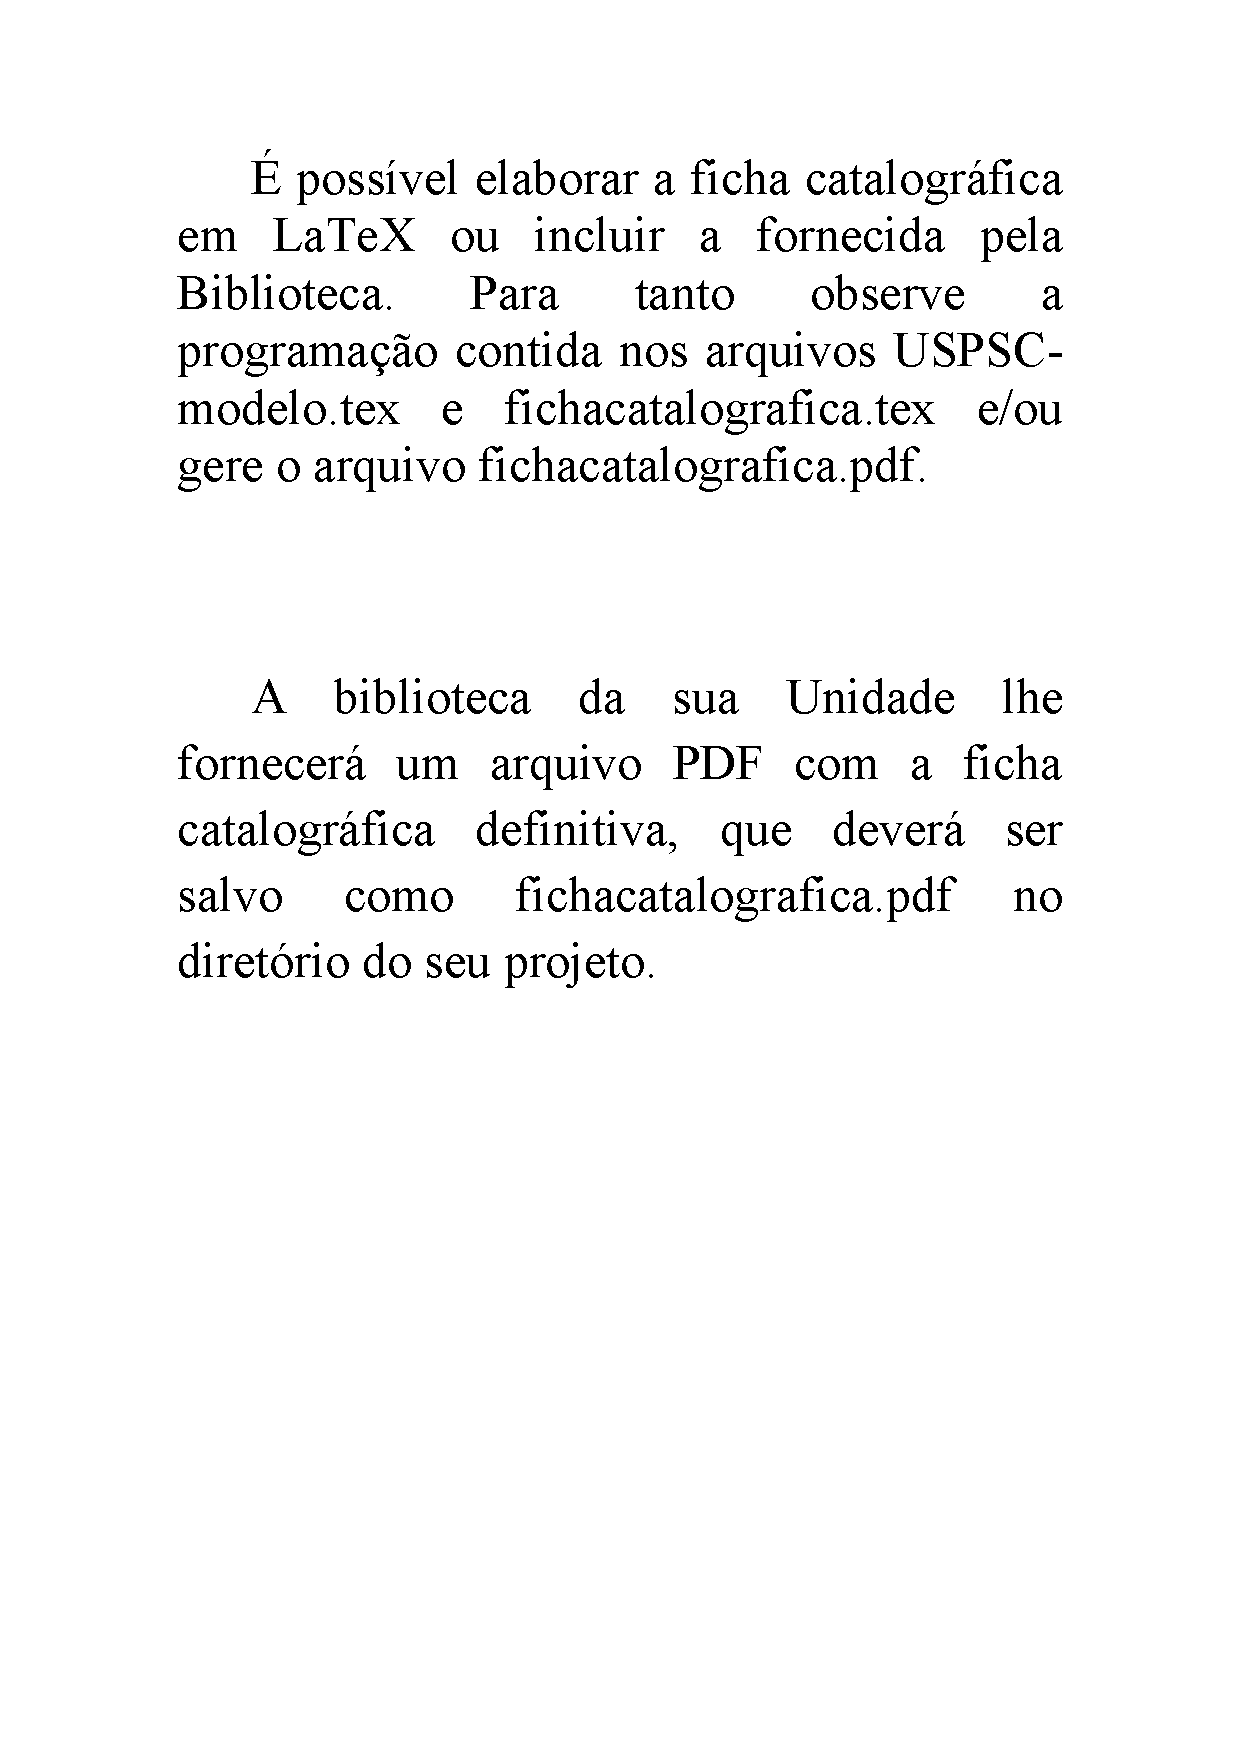
\includepdf{USPSC-Tese-pre-textual/fichacatalografica.pdf} 
% Se você optar por elaborar a ficha catalográfica, deverá 
% incluir uma % antes da linha % antes
% do comando % ---
% Inserir a ficha bibliografica
% ---
% Isto é um exemplo de Ficha Catalográfica, ou ``Dados internacionais de
% catalogação-na-publicação''. Você pode utilizar este modelo como referência. 
% Porém, provavelmente a biblioteca da sua universidade lhe fornecerá um PDF
% com a ficha catalográfica definitiva após a defesa do trabalho. Quando estiver
% com o documento, salve-o como PDF no diretório do seu projeto e substitua todo
% o conteúdo de implementação deste arquivo pelo comando abaixo:
%
\begin{fichacatalografica}
	\hspace{-1.4cm}
	\imprimirnotaautorizacao \\ \\
	%\sffamily
	\vspace*{\fill}					% Posição vertical
	\begin{center}					% Minipage Centralizado
		\imprimirnotabib \\
\begin{table}[htb]
	\scriptsize
	\centering	
	\begin{tabular}{|p{0.9cm} p{8.7cm}|}
		\hline
	      & \\
		  &	  \imprimirautorficha     \\
		
		 \imprimircutter & 
							\hspace{0.4cm}\imprimirtitulo~  / ~\imprimirautor~ ;  ~\imprimirorientadorcorpoficha. -- 	\imprimirlocal, \imprimirdata.   \\
		
		  &  % Para incluir nota referente à versão corrigida no corpo da ficha,
			  % incluir % no início da linha acima e tirar a % do início da linha abaixo
			  %	\hspace{0.4cm} \imprimirtitulo~  / ~\imprimirautor~ ; ~\imprimirorientadorcorpoficha~- ~\imprimirnotafolharosto. -- \imprimirlocal, \imprimirdata.  \\
		
			\hspace{0.4cm}\pageref{LastPage} p. : il. (algumas color.) ; 30 cm.\\ 
		  & \\
		  & 
		    \hspace{0.4cm}\imprimirnotaficha ~--~ 
						  \imprimirunidademin, 
						  \imprimiruniversidademin, 
		                  \imprimirdata. \\ 
		  & \\                 
		   % Para incluir nota referente à versão corrigida em notas,
		    % incluir uma % no início da linha acima e	
		    % tirar a % do início da linha abaixo
		    % & \hspace{0.4cm}\imprimirnotafolharosto \\ 
		  & \\ 
		  & \hspace{0.4cm}1. LaTeX. 2. abnTeX. 3. Classe USPSC. 4. Editoração de texto. 5. Normalização da documentação. 6. Tese. 7. Dissertação. 8. Documentos (elaboração). 9. Documentos eletrônicos. I. \imprimirorientadorficha. 
		   II. Título. \\
	
		     %Se houver co-orientador, inclua % antes da linha (antes de II. Título.) 
		     %          e tire a % antes do comando abaixo 
		     %III. Título. \\   
		  \hline
	\end{tabular}
\end{table}
	\end{center}
\end{fichacatalografica}
% ---

 
% e retirar o % do comando abaixo
%% ---
% Inserir a ficha bibliografica
% ---
% Isto é um exemplo de Ficha Catalográfica, ou ``Dados internacionais de
% catalogação-na-publicação''. Você pode utilizar este modelo como referência. 
% Porém, provavelmente a biblioteca da sua universidade lhe fornecerá um PDF
% com a ficha catalográfica definitiva após a defesa do trabalho. Quando estiver
% com o documento, salve-o como PDF no diretório do seu projeto e substitua todo
% o conteúdo de implementação deste arquivo pelo comando abaixo:
%
\begin{fichacatalografica}
	\hspace{-1.4cm}
	\imprimirnotaautorizacao \\ \\
	%\sffamily
	\vspace*{\fill}					% Posição vertical
	\begin{center}					% Minipage Centralizado
		\imprimirnotabib \\
\begin{table}[htb]
	\scriptsize
	\centering	
	\begin{tabular}{|p{0.9cm} p{8.7cm}|}
		\hline
	      & \\
		  &	  \imprimirautorficha     \\
		
		 \imprimircutter & 
							\hspace{0.4cm}\imprimirtitulo~  / ~\imprimirautor~ ;  ~\imprimirorientadorcorpoficha. -- 	\imprimirlocal, \imprimirdata.   \\
		
		  &  % Para incluir nota referente à versão corrigida no corpo da ficha,
			  % incluir % no início da linha acima e tirar a % do início da linha abaixo
			  %	\hspace{0.4cm} \imprimirtitulo~  / ~\imprimirautor~ ; ~\imprimirorientadorcorpoficha~- ~\imprimirnotafolharosto. -- \imprimirlocal, \imprimirdata.  \\
		
			\hspace{0.4cm}\pageref{LastPage} p. : il. (algumas color.) ; 30 cm.\\ 
		  & \\
		  & 
		    \hspace{0.4cm}\imprimirnotaficha ~--~ 
						  \imprimirunidademin, 
						  \imprimiruniversidademin, 
		                  \imprimirdata. \\ 
		  & \\                 
		   % Para incluir nota referente à versão corrigida em notas,
		    % incluir uma % no início da linha acima e	
		    % tirar a % do início da linha abaixo
		    % & \hspace{0.4cm}\imprimirnotafolharosto \\ 
		  & \\ 
		  & \hspace{0.4cm}1. LaTeX. 2. abnTeX. 3. Classe USPSC. 4. Editoração de texto. 5. Normalização da documentação. 6. Tese. 7. Dissertação. 8. Documentos (elaboração). 9. Documentos eletrônicos. I. \imprimirorientadorficha. 
		   II. Título. \\
	
		     %Se houver co-orientador, inclua % antes da linha (antes de II. Título.) 
		     %          e tire a % antes do comando abaixo 
		     %III. Título. \\   
		  \hline
	\end{tabular}
\end{table}
	\end{center}
\end{fichacatalografica}
% ---


% As informações que compõem a ficha catalográfica estão 
% definidos no arquivo USPSC-pre-textual-UUUU.tex
% ---


% ---
% ---
% Inserir errata
% ---

\begin{errata}
	\OnehalfSpacing 			
	A errata é um elemento opcional, que consiste de uma lista de erros da obra, precedidos pelas folhas e linhas onde eles ocorrem e seguidos pelas correções correspondentes. Deve ser inserida logo após a folha de rosto e conter a referência do trabalho para facilitar sua identificação, conforme a ABNT NBR 14724 \cite{nbr14724}.
	
	Modelo de Errata:
		
	\begin{flushleft} 
			\setlength{\absparsep}{0pt} % ajusta o espaçamento da referência	
			\SingleSpacing 
			\imprimirautorabr~ ~\textbf{\imprimirtitulo}.	\imprimirdata. \pageref{LastPage}p. 
			%Substitua p. por f. quando utilizar oneside em \documentclass
			%\pageref{LastPage}f.
			\imprimirtipotrabalho~-~\imprimirinstituicao, \imprimirlocal, \imprimirdata. 
 	\end{flushleft}
\vspace{\onelineskip}
\OnehalfSpacing 
\center
\textbf{ERRATA}
\vspace{\onelineskip}
\OnehalfSpacing 
\begin{table}[htb]
	\center
	\footnotesize
	\begin{tabular}{p{1.4cm} p{1cm} p{3cm} p{3cm} }
		\hline
		\textbf{Folha} & \textbf{Linha}  & \textbf{Onde se lê}  & \textbf{Leia-se}  \\
			\hline
			1 & 10 & auto-conclavo & autoconclavo\\
		\hline
	\end{tabular}
\end{table}


\end{errata}
% ---

% ---
% Inserir folha de aprovação
% ---

% A Folha de aprovação é um elemento obrigatório da NBR 4724/2011 (seção 4.2.1.3). 
% Após a defesa/aprovação do trabalho, gere o arquivo folhadeaprovacao.pdf da página assinada pela banca 
% e iclua o arquivo utilizando o comando abaixo:
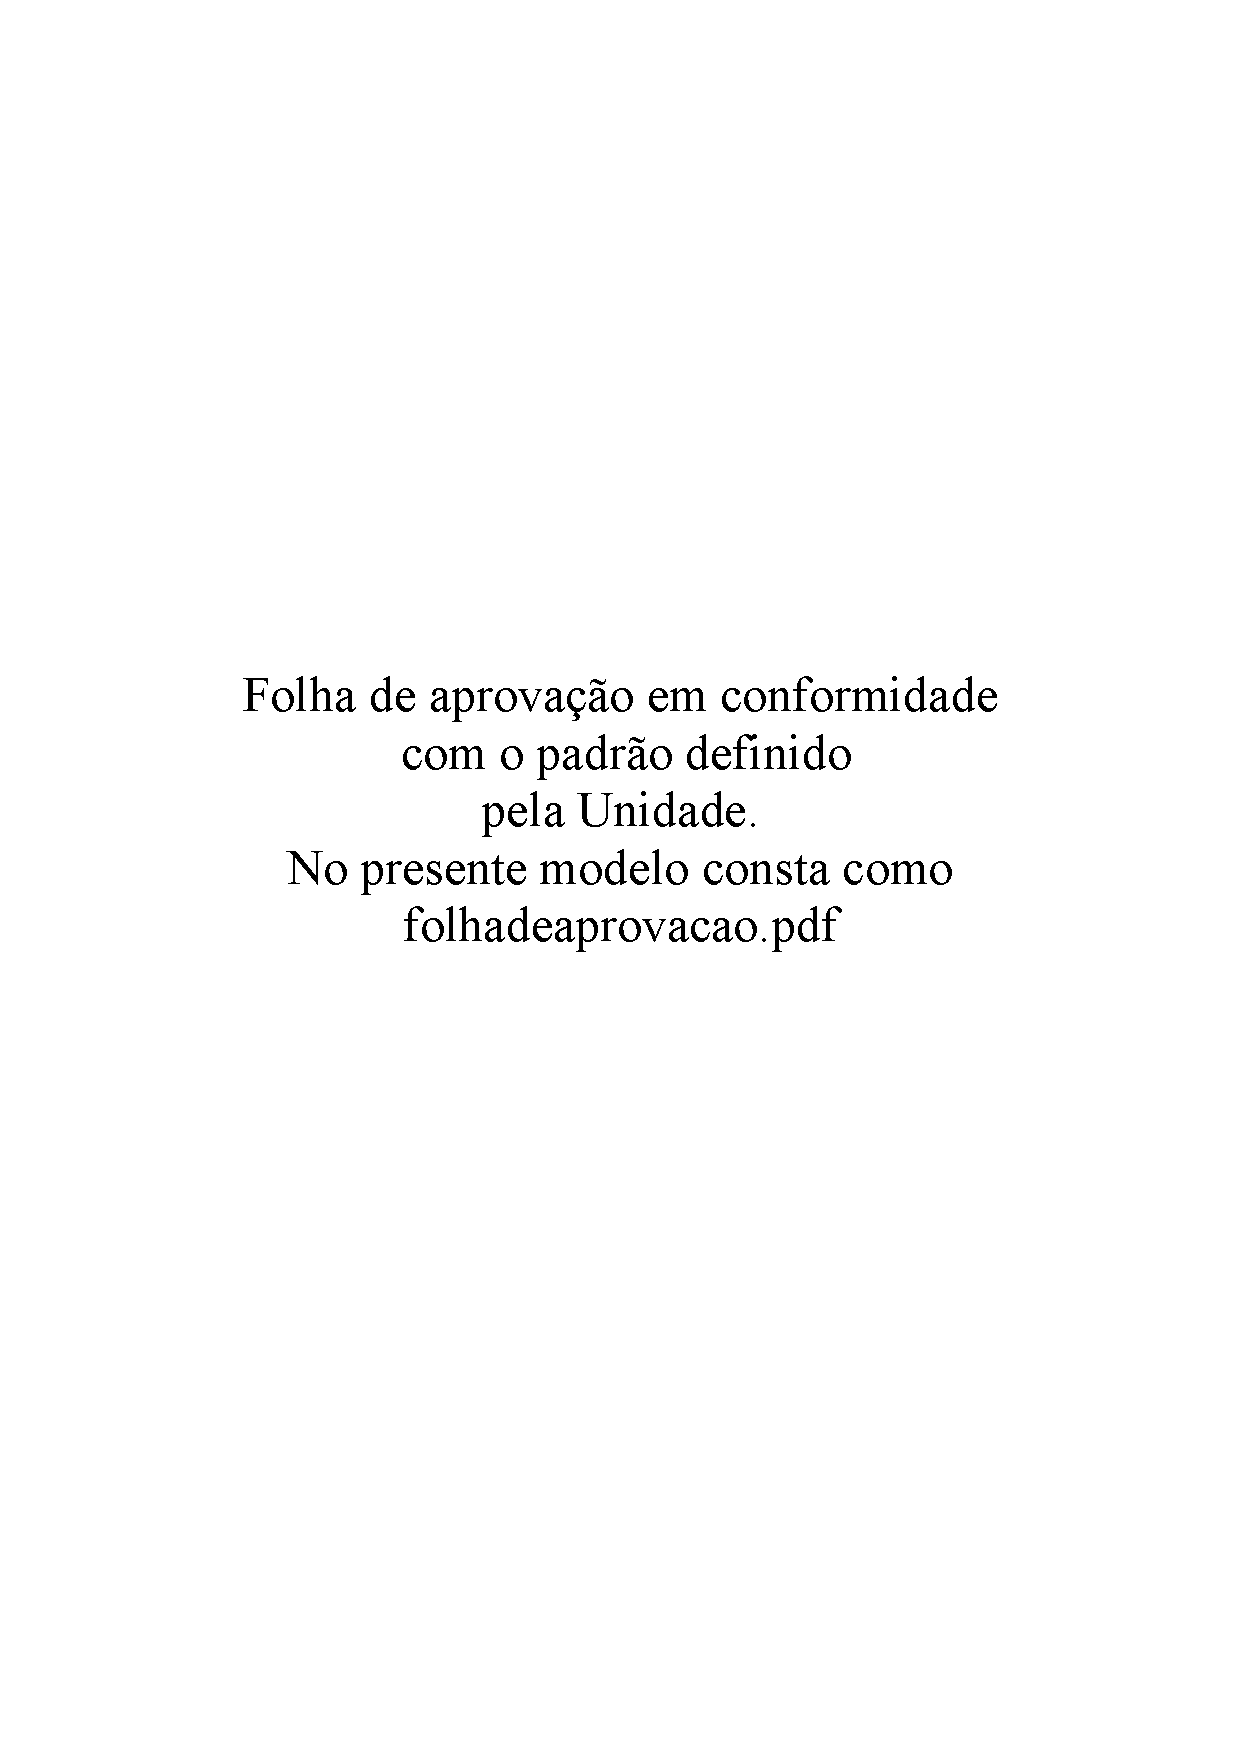
\includepdf{folhadeaprovacao.pdf}
% Alternativa para a Folha de Aprovação:
% Se for a sua opção elaborar uma folha de aprovação, insira uma % antes do comando acima que inclui o arquivo folhadeaprovacao.pdf,
% tire o % do comando abaixo e altere o arquivo folhadeaprovacao.tex conforme suas necessidades
%% Alternativa para a Folha de Aprova��o 
% Se esta for a sua op��o, exclua inclus�o feita acima do arquivo folhadeaprovacao.pdf
%
\begin{folhadeaprovacao}
  \begin{center}
       {\ABNTEXchapterfont\bfseries\large\imprimirautor}
	 \vspace*{2cm}
   
    \begin{center}
      \ABNTEXchapterfont\bfseries\Large\imprimirtitulo
    \end{center}
		\vspace*{2cm}
		\hspace{.45\textwidth}
    \begin{minipage}{.5\textwidth}
        \imprimirpreambulo
    \end{minipage}
		\vspace*{2cm}
    %\vspace*{\fill}
	\end{center}

  \begin{center}
	  {\ABNTEXchapterfont\bfseries\large\ {Data de defesa: 02 de outubro de 2015} \\}
		\vspace*{\fill}
	  {\ABNTEXchapterfont\bfseries\large\ {Comiss\~ao Julgadora:} \\}
		%Trabalho aprovado. \imprimirlocal, 2 de outubro de 2015:
		
		%\assinatura{\textbf{\imprimirorientador} \\ Orientador} 
		\assinatura{\textbf{\imprimirorientador} \\}
    % Se for ORIENTADOR, inclua % no in�cio do comando abaixo e tire a % do pr�ximo comando 
		\renewcommand{\orientadorname}{Orientadora}
		%\renewcommand{\orientadorname}{Orientador}

		\imprimirorientadorRotulo
		\par
		\assinatura{\textbf{Professor} \\ Convidado1}
	
		\assinatura{\textbf{Professor} \\ Convidado2}
		%\assinatura{\textbf{Professor} \\ Convidado3}
		%\assinatura{\textbf{Professor} \\ Convidado4}
		%\begin{center}
		\vspace*{\fill}
   	{\ABNTEXchapterfont\bfseries\large\imprimirlocal}
    \par
    {\ABNTEXchapterfont\bfseries\large\imprimirdata}
\end{center}
\end{folhadeaprovacao}
% ---


\includepdf{PaginaEmBranco.pdf}

% ---
% Dedicatória
% ---
%% USPSC-Dedicatória.tex
% ---
% Dedicatória
% ---
\begin{dedicatoria}
   \vspace*{\fill}
   \centering
   \noindent
   \textit{ Este trabalho é dedicado aos alunos da USP, como uma contribuição\\
  das Bibliotecas do Campus USP de São Carlos para o desenvolvimento\\
	e disseminação da pesquisa científica da Universidade.} \vspace*{\fill}
\end{dedicatoria}
% ---
% ---

% ---
% Agradecimentos
% ---
%% Agradecimentos.tex
% ---
% Agradecimentos
% ---=====
\begin{agradecimentos}
	A motivação para o desenvolvimento da classe USPSC e dos modelos de trabalhos acadêmicos foi decorrente de solicitações de usuários das Bibliotecas do Campus USP de São Carlos. A versão 2.0 do Pacote USPSC é composto da \textbf{Classe USPSC}, do \textbf{Modelo para TCC em \LaTeX\ utilizando a classe USPSC} e do \textbf{Modelo para teses e dissertações em \LaTeX\ utilizando a classe USPSC}.
	
	O Modelo para TCC está disponível inicialmente apenas para EESC e será estendido às demais Unidades de Ensino do Campus USP de São Carlos a medida que as mesmas definirem seus padrões.
	
	O Grupo desenvolvedor do Pacote USPSC agradece especialmente ao Luis Olmes, doutorando do Instituto de Ciências Matemáticas e de Computação (ICMC) da Universidade de São Paulo (USP), pelas primeiras orientações sobre o \LaTeX\ . 
	
	Agradecemos ao Lauro César Araujo pelo desenvolvimento da classe  \abnTeX, modelos canônicos e tantas outras contribuições que nos permitiu o desenvolvimento da classe USPSC e seus modelos.
	
	Os nossos agradecimentos aos integrantes do primeiro
	projeto abn\TeX\, Gerald Weber, Miguel Frasson, Leslie H. Watter, Bruno Parente Lima, Flávio de Vasconcellos Corrêa, Otavio Real
	Salvador, Renato Machnievscz, e a todos que contribuíram para que a produção de trabalhos acadêmicos em conformidade com
	as normas ABNT com \LaTeX\ fosse possível.
	
	Agradecemos ao grupo de usuários
	\emph{latex-br}{\url{http://groups.google.com/group/latex-br}}, aos integrantes do grupo
	\emph{\abnTeX}{\url{http://groups.google.com/group/abntex2}  e \url{http://www.abntex.net.br/}}~que contribuem para a evolução do \abnTeX.
\end{agradecimentos}
% ---
% ---

% ---
% Epígrafe
% ---
\begin{epigrafe}
    \vspace*{\fill}
	\begin{flushright}
		\textit{``O estudo, a busca da verdade e da beleza são domínios \\
		em que nos é consentido sermos crianças por toda a vida.''\\
		Albert Einstein}
	\end{flushright}
\end{epigrafe}
% ---

% A T E N Ç Ã O
% Se o idioma do texto for em inglês, o abstract deve preceder o resumo
% resumo em português
%
% Resumo
% ---
%% Resumo.tex
% ---
% Resumo
% ---
\setlength{\absparsep}{18pt} % ajusta o espaçamento dos parágrafos do resumo		

\begin{resumo}[Resumo]

\begin{otherlanguage*}{brazil}

\begin{flushleft} 
	\setlength{\absparsep}{0pt} % ajusta o espaçamento da referência	
	\SingleSpacing 
	\imprimirautorabr~ ~\textbf{\imprimirtitulo}.	\imprimirdata. \pageref{LastPage}p. 
	%Substitua p. por f. quando utilizar oneside em \documentclass
	%\pageref{LastPage}f.
	\imprimirtipotrabalho~-~\imprimirinstituicao, \imprimirlocal, \imprimirdata. 
\end{flushleft}

\OnehalfSpacing 			

O presente trabalho prop\~oe o desenvovlimento de um \textit{software} voltado para a identifica\c{c}\~ao de modelos de sistemas n\~ao-lineares, com enfoque em plantas e\'olicas. O modelo escolhido para plantas e\'olicas \'e bem consolidado na literatura, sendo capaz de representar o comportamento de geradores mais utilizados nas instala\c{c}\~oes deste tipo tanto durante o regime permanente quanto em transit\'orios. O m\'etodo utilizado para a identifica\c{c}\~ao do modelo \'e constitu\'ido por dois algoritmos de otimiza\c{c}\~ao. Primeiramente, \'e empregada uma abordagem heur\'istica, baseada em Otimiza\c{c}\~ao por Mapeamento de M\'edia-Vari\^ancia, a fim de reduzir a regi\~ao de busca dos par\^ametros em torno de uma poss\'ivel solu\c{c}\~ao. Em seguida, lan\c{c}a-se m\~ao de um algoritmo n\~ao-linear, baseado no M\'etodo de Sensibilidade de Trajet\'oria, para realizar os ajustes finais nos valores dos par\^ametros. A valida\c{c}\~ao do m\'etodo ser\'a feita utilizando medidas de sistemas simulados. Com o intuito de facilitar a experi\^encia do usu\'ario com o programa, ser\'a desenvolvida uma interface gr\'afica para o \textit{software}. Tanto as rotinas para identifica\c{c}\~ao de modelos quanto a interface gr\'afica ser\~ao desenvolvidas em Python.
 

\textbf{Palavras-chave}: Identifica\c{c}\~ao de modelos. Plantas e\'olicas. MVMO. Sensibilidade de trajet\'oria. Python.

\end{otherlanguage*}

\end{resumo}
% ---

% Abstract
% ---
%% Abstract.tex
% ---
% Abstract
% ---
\autor{Silva, M. J.}
\begin{resumo}[Abstract]
 \begin{otherlanguage*}{english}
	\begin{flushleft} 
		\setlength{\absparsep}{0pt} % ajusta o espaçamento dos parágrafos do resumo		
 		\SingleSpacing 
 		\imprimirautorabr~ ~\textbf{\imprimirtitleabstract}.	\imprimirdata.  \pageref{LastPage}p. 
		%Substitua p. por f. quando utilizar oneside em \documentclass
		%\pageref{LastPage}f.
		\imprimirtipotrabalho~-~\imprimirinstituicao, \imprimirlocal, 	\imprimirdata. 
 	\end{flushleft}
\OnehalfSpacing
This project proposes the development of a software for non-linear system's model identification, focusing on wind power plants. The chosen model  for wind power plants is well-known in the literature and is capable of representing the most common wind turbine type during both steady-state and transients. The method applied to identify the model is composed of two optimization algorithms. At the begining of the process, an heuristic approach based on Mean-Variance Mapping Optimization is used in order to reduce the parameter's search region around a possible solution. Afterward, a non-linear algorithm based on Trajectory Sensitivity is used to fine-tune the parameters. The method validation will be made using data from simulated systems. Also, a guided user interface will be developed for this application, aiding new users. All coding for this project will be made in Python.


\textbf{Keywords}: Model identification. Wind power plants. MVMO. Trajectory sensitivity. Python.
 \end{otherlanguage*}
\end{resumo}

% ---

% ---
% inserir lista de figurass
% ---
\pdfbookmark[0]{\listfigurename}{lof}
\listoffigures*
\cleardoublepage
% ---

% ---
% inserir lista de tabelas
% ---
\pdfbookmark[0]{\listtablename}{lot}
\listoftables*
\cleardoublepage
% ---

% ---
% inserir lista de quadros
% ---
\pdfbookmark[0]{\listofquadroname}{loq}
\listofquadro*
\cleardoublepage
% ---

% ---
% inserir lista de abreviaturas e siglas
% ---
\begin{siglas}
    \item[ABNT] Associação Brasileira de Normas Técnicas
    \item[abnTeX] ABsurdas Normas para TeX
	\item[EESC] Escola de Engenharia de São Carlos
	\item[IAU] Instituto de Arquitetura e Urbanismo
	\item[IBGE] Instituto Brasileiro de Geografia e Estatística
	\item[ICMC] Instituto de Ciências Matemáticas e de Computação
	\item[IFSC] Instituto de Física de São Carlos
	\item[IQSC] Instituto de Química de São Carlos
	\item[PDF] Portable Document Format
	\item[TCC] Trabalho de Conclusão de Curso
	\item[USP] Universidade de São Paulo
	\item[USPSC] Campus USP de São Carlos
	
\end{siglas}
% ---

% ---
% inserir lista de símbolos
% ---
\begin{simbolos}
  \item[$ \Gamma $] Letra grega Gama
  \item[$ \Lambda $] Lambda
  \item[$ \zeta $] Letra grega minúscula zeta
  \item[$ \in $] Pertence
\end{simbolos}
% ---
% ---
% inserir o sumario
% ---
\pdfbookmark[0]{\contentsname}{toc}
\tableofcontents*
\cleardoublepage
% ---
% ----------------------------------------------------------
% ELEMENTOS TEXTUAIS
% ----------------------------------------------------------
\textual
% Os capítulos são inseridos como arquivos externos 

% Capítulo 1 - Introdução
% ---
%% USPSC-Introducao.tex

% ----------------------------------------------------------
% Introdução (exemplo de capítulo sem numeração, mas presente no Sumário)
% ----------------------------------------------------------
\chapter[Introduction]{Introduction}
\label{ch: Intro}

During the last decade, the world has seen an increase in participation of renewable sources in power generation, leaded mainly by wind and solar energy. These green technologies provide an alternative to sources based on fossil fuel, lowering pollution levels and reducing greenhouse gas emissions. On the other hand, the power output from these sources rely on weather conditions and can't be fully controlled.

This increase is seen worldwide, as part of policies to reduce the human impact on climate and the environment. This `renewable wave' is leaded mainly by European countries, specially in the European Union (EU), United States (US) and China. In particular, EU has set in 2010 a strategy plan to reduce its greenhouse emissions by at least 20\% compared to 1990 levels and increase the share of renewable sources to at least 20\% by 2020 \cite{Europe2020}.

Brazil does not lag far behind EU regarding renewable sources policies. In 2002, the country passed a bill that, among other actions, creates the Program of Incentive to Alternative Electric Energy Sources (PROINFA). This program aims to increase the share of wind, solar, small hydro and biomass energy production. The final goal is to have these energy sources corresponding to 10\% of Brazil's annual energy consumption by 2024 \cite{Brazil2002}.

\section{Wind Energy}

Those policies stimulated the increase of wind energy participation, reaching a scenario where it is the main energy source of some countries. In the EU, wind energy alone generated 362 TWh in 2018, covering 14\% of the electricity demand, a share 2\% higher than 2017. Among the EU countries, Denmark leads in this sector, with 41\% of its demand supplied by wind power plants, followed by Ireland (28\%), Portugal (24\%) and Germany (21\%). The total installed capacity across the 28 EU countries is 178.8 GW, with Germany in first position, with a total installed capacity of 59.3 GW, followed by Spain and the United Kingdom (UK), with 23.5 and 21.0 GW installed, respectively \cite{WindEurope2019}. Figure \ref{fig: EUrank} displays the detailed percentage of electricity demand covered by wind in the EU.

\begin{figure}[]
	\caption{Share of electricity demand in the EU covered by wind energy during 2018}
	\begin{center}
		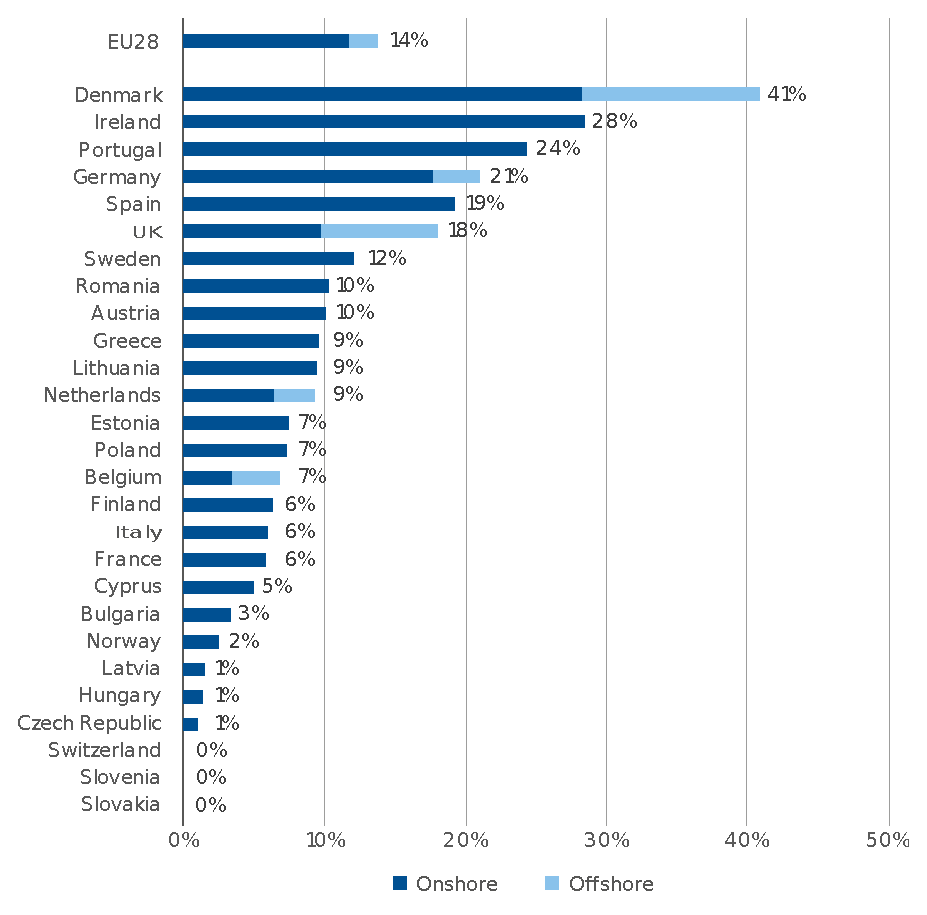
\includegraphics[scale=0.65]{Images/EUrank.eps}
	\end{center}
	\label{fig: EUrank}
	\legend{Source: Wind Europe, 2019}
\end{figure}

In Brazil, wind energy contributed with 42.4 TWh during 2017, resulting in a participation share of 7.2\%. For comparison, Itaipu, the largest power plant in Brazil, has produced 96.4 TWh during the same period. But, while other sources, such as hydro and coal, had its share lowered, wind energy had the highest variation among sources comparing to 2016, increasing its contribution by 26.5\% \cite{EPE2018}. 

In therms of installed capacity, wind power plants appear in \nth{2} place, with 14.7 GW installed, only behind hydro power plants \cite{ABEEolica2018}, as shown in Figure \ref{fig: BRshare}. However, there is still plenty of energy yield for this source to be explored. In \cite{Atlas2001} is shown that Brazil has potential to generate 272.2 TWh per year, with an installed capacity of 143.5 GW. The Northeast Region has the higher potential, with an annual energy yield of 144.3 TWh and potential to host up to 75.0 GW . Also, the wind regime in the Northeast Region is complimentary to the water regime of the main river responsible to power generation in the region, as presented by Figure \ref{fig: WindWater}. This characteristic would help controlling reservoir water level during dry season, an important resource not only for power generation, but also irrigation of crops and water supply \cite{ANEEL2005}.

\begin{figure}[]
	\caption{Electricity generation in Brazil by source}
	\begin{center}
		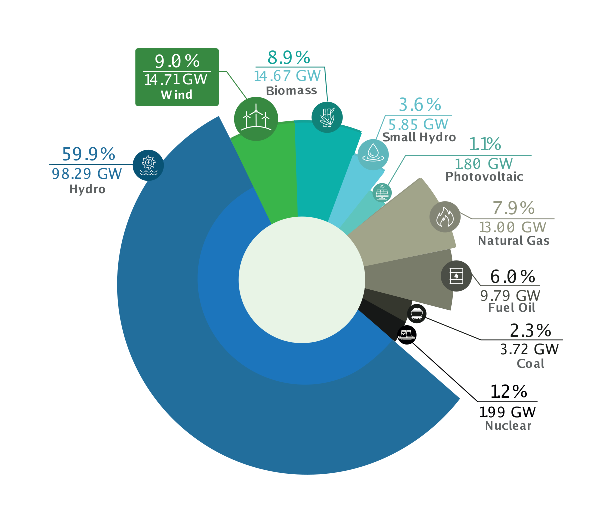
\includegraphics[scale=0.8]{Images/BRshare19.eps}
	\end{center}
	\label{fig: BRshare}
	\legend{Source: ABEE\'olica, 2018}
\end{figure}

\begin{figure}[]
	\caption{Wind and water regime in the Brazilian Northeast Region}
	\begin{center}
		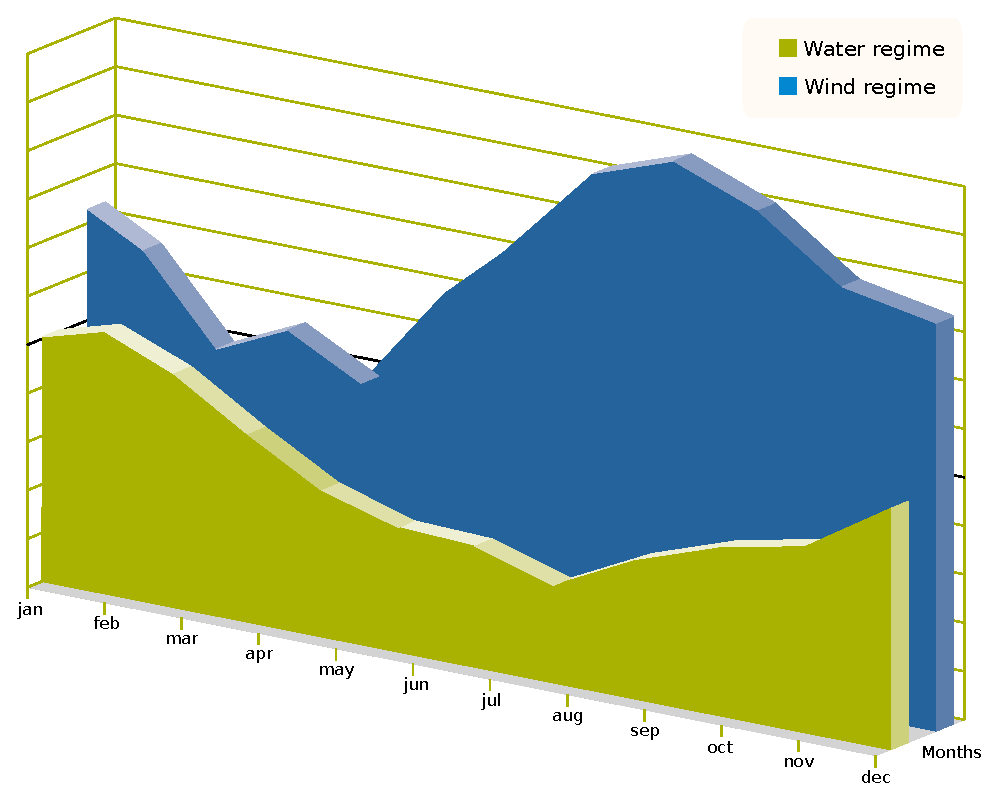
\includegraphics[scale=0.5]{Images/WindWater.eps}
	\end{center}
	\label{fig: WindWater}
	\legend{Source: ANEEL, 2005}
\end{figure}

With all this information in hand, it is only reasonable to assume that wind energy will increase its participation in electricity generation. But, in order to allow this growth, studies about how wind generators and power plants behave during faults in the grid are needed.

\section{Wind Turbine Model}

With a growing share of energy covered by wind, system operators must consider how wind turbines affect the system stability during faults and maneuvers. To do so, mathematical models capable of describing these machines' behaviour are crucial. Obtaining these models, on the other hand, is not an easy task, due to considerable amount of wind turbines in large power plants, with different manufacturers, technologies, sizes, distances from point of connection and wind conditions. Thus, a model that describes well a particular turbine in a power plant, won't necessarily work for its neighboring generators. Also, due to industrial secrecy, manufacturers provide little or no information about how their turbines behave. Furthermore, having one model for every wind turbine within a power plant would result in a mathematical problem with high complexity and computational cost \cite{Erlich2012}.

To address this problem, studies such as \cite{Muljadi2008}, \cite{Ellis2011}, \cite{council2008wecc} and \cite{Asmine2011}, motivated specially by the Institute of Electrical and Electronics Engineers (IEEE) and the Western Electricity Coordinating Council (WECC), developed generic models able to predict the behaviour of entire wind power plants. Such models reduced the problem complexity, since they were composed of a single equivalent generator. A two-machine model is needed only in rare cases, such as when the wind power plant is composed of two or more types of wind turbines \cite{Ellis2011}.

These studies have also shown that commercial wind turbine generators (WTG) could be sorted into four basic types, according to its technology \cite{Ellis2011}. These types are described in the following subsections.

\subsection{Type-1 Wind Turbine Generator}

The first type of wind turbine generator is composed of a Squirrel Cage Induction Generator (SCIG) connected to a wind turbine through a controlled gearbox, as displayed in Figure \ref{fig: WTG1}. Due to its torque-speed characteristics, generators of this type operate at constant rotor speed, requiring robust controllers on gearbox and blade. Besides, as usual to any induction generator, the SCIG absorbs reactive power during operation. Thus, capacitors are often employed for power faction correction purposes. Moreover, type-1 generators limit aerodynamic power by varying the pitch angle of their blades, imposing great mechanical stress on blades, shafts and gears, demanding a robust mechanical design and preventing these generators to operate above certain wind speed \cite{Ellis2011}. 

\begin{figure}[h]
	\caption{Representation of Type-1 Wind Turbine Generator}
	\begin{center}
		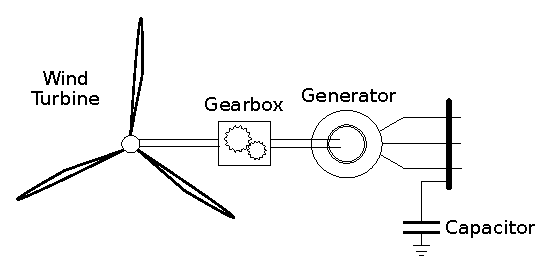
\includegraphics[scale=1]{Images/Type1WTG.eps}
	\end{center}
	\label{fig: WTG1}
\end{figure}

\subsection{Type-2 Wind Turbine Generator}

Similarly to Type-1 WTG, Type-2 Wind Turbine Generators are composed of an asynchronous machine connected to a wind turbine via gearbox, but, instead of SCIG, Wound Rotor Induction Generator (WRIG) are used to convert kinetic energy into electricity. The WRIG has access to its rotor windings, allowing to vary the rotor resistance. As a direct consequence, this machine can operate in different wind speeds by adjusting its torque-speed curve as needed \cite{Ellis2011}. Therefore, Type-2 WTG have a WRIG with a variable resistance connected to its rotor terminals, as shown in Figure \ref{fig: WTG2}.

\begin{figure}[h]
	\caption{Representation of Type-2 Wind Turbine Generator}
	\begin{center}
		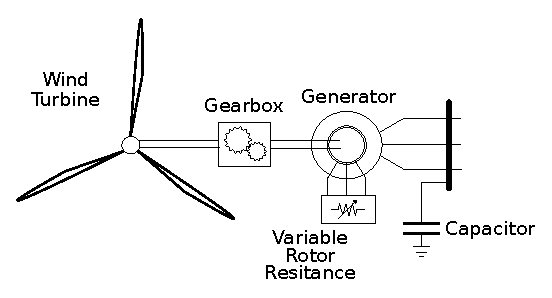
\includegraphics[scale=1]{Images/Type2WTG.eps}
	\end{center}
	\label{fig: WTG2}
\end{figure}

This type of generator has then three speed control systems, with rotor resistance control responding to rapid changes in speed, gearbox control for medium variations and pitch control for slow changes. These control system work together to maintain power output constant and reduce mechanical stress on components. The effects on the torque-speed curve caused by different rotor resistances are shown in Figure \ref{fig: Tw}. For a fixed power, increasing rotor resistance increases the speed needed on the shaft, allowing the wind turbine to operate above rated wind speed. However, the speed range is only $\pm 10\%$ of rated slip. Also, this machine still needs a reactive compensation circuit on its terminals \cite{Muljadi2010}.

\begin{figure}[h]
	\caption{Torque-speed curve}
	\begin{center}
		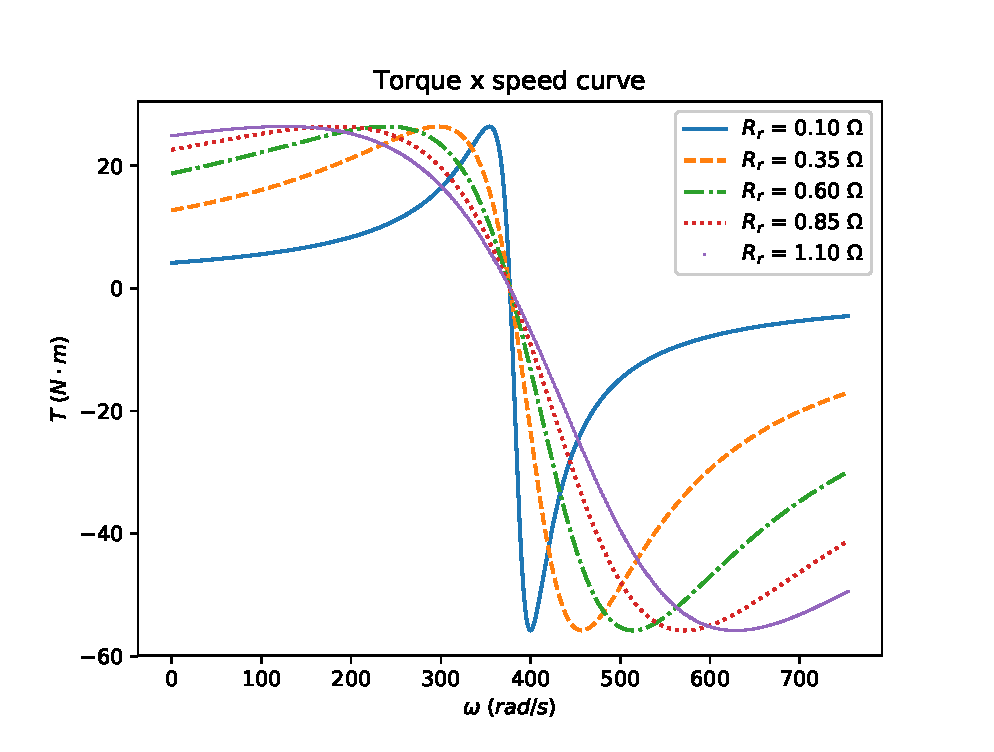
\includegraphics[scale=.7]{Images/Tw_curve.eps}
	\end{center}
	\label{fig: Tw}
\end{figure}

\subsection{Type-3 Wind Turbine Generator}

A Type-3 Wind Turbine Generator, often called Doubly Fed Induction Generator (DFIG), is also composed of a wound rotor machine connected to a wind turbine. But, instead of varying rotor resistance, a DFIG has its rotor supplied with AC voltage by a back-to-back frequency converter, as displayed in Figure \ref{fig: WTG3}. By varying the voltage frequency on the rotor circuit, the generator is able to supply power to the grid in a wider range of wind speed, reaching up to $\pm 30\%$ of rated slip. In addition, the converter can control both real and reactive power independently, ending the necessity of capacitors \cite{Muljadi2010}. Since approximately 30\% of rated power flows through the rotor windings, power electronics components have lower specifications and don't have great impact on overall costs. On the other hand, these generators need regular maintenance due to slip rings, brushes and gearbox, preventing its use in offshore applications \cite{Yaramasu2015}.

\begin{figure}[h]
	\caption{Representation of Type-3 Wind Turbine Generator}
	\begin{center}
		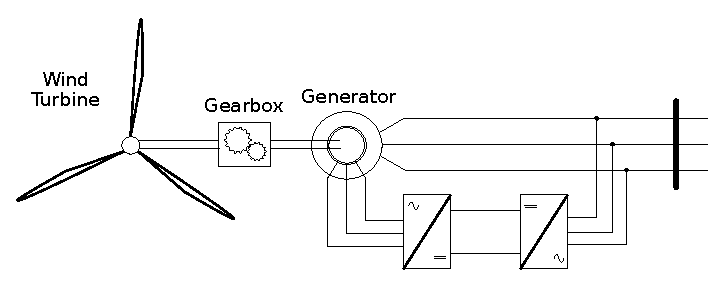
\includegraphics[scale=1]{Images/Type3WTG.eps}
	\end{center}
	\label{fig: WTG3}
\end{figure}

\subsection{Type-4 Wind Turbine Generator}

The last type of wind turbine generator, also called Full-Converter Generator, is composed of a electrical machine connected to the grid through a back-to-back frequency converter. The converter will operate converting the electrical frequency generated to standard, allowing this type of WTG to operate in a large range of wind speed (up to almost 100\% of rated slip). Due to the converter operation, connection to the wind turbine can be made directly or via gearbox. Likewise, it allows the use of synchronous and asynchronous electrical machines as generator, with Permanent Magnet Synchronous Generator (PMSG), Electrical Excited Synchronous Generator (EESG) and SCIG being most common, because of cost and maintenance purposes. Similar to DFIG, full-converter generators are able to control real and reactive power injected into the grid. However, since all power generated must flow through the power electronics, the overall cost of these generators is usually higher \cite{Yaramasu2015}. Figure \ref{fig: WTG4} depicts a typical Type-4 Wind Turbine Generator.

\begin{figure}[h]
	\caption{Representation of Type-4 Wind Turbine Generator}
	\begin{center}
		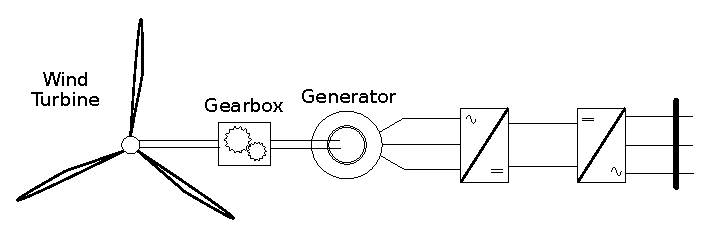
\includegraphics[scale=1]{Images/Type4WTG.eps}
	\end{center}
	\label{fig: WTG4}
\end{figure}

Figure \ref{fig: WindShare} shows the evolution of share in installed capacity onshore for each generator type. The data shows how SCIG and WRIG lost space in the segment and how DFIG and Full-Converter Generators' participation rose, dominating the global market \cite{Magagna2017}.

\begin{figure}[h]
	\caption{Share of installed capacity for each wind turbine generator type}
	\begin{center}
		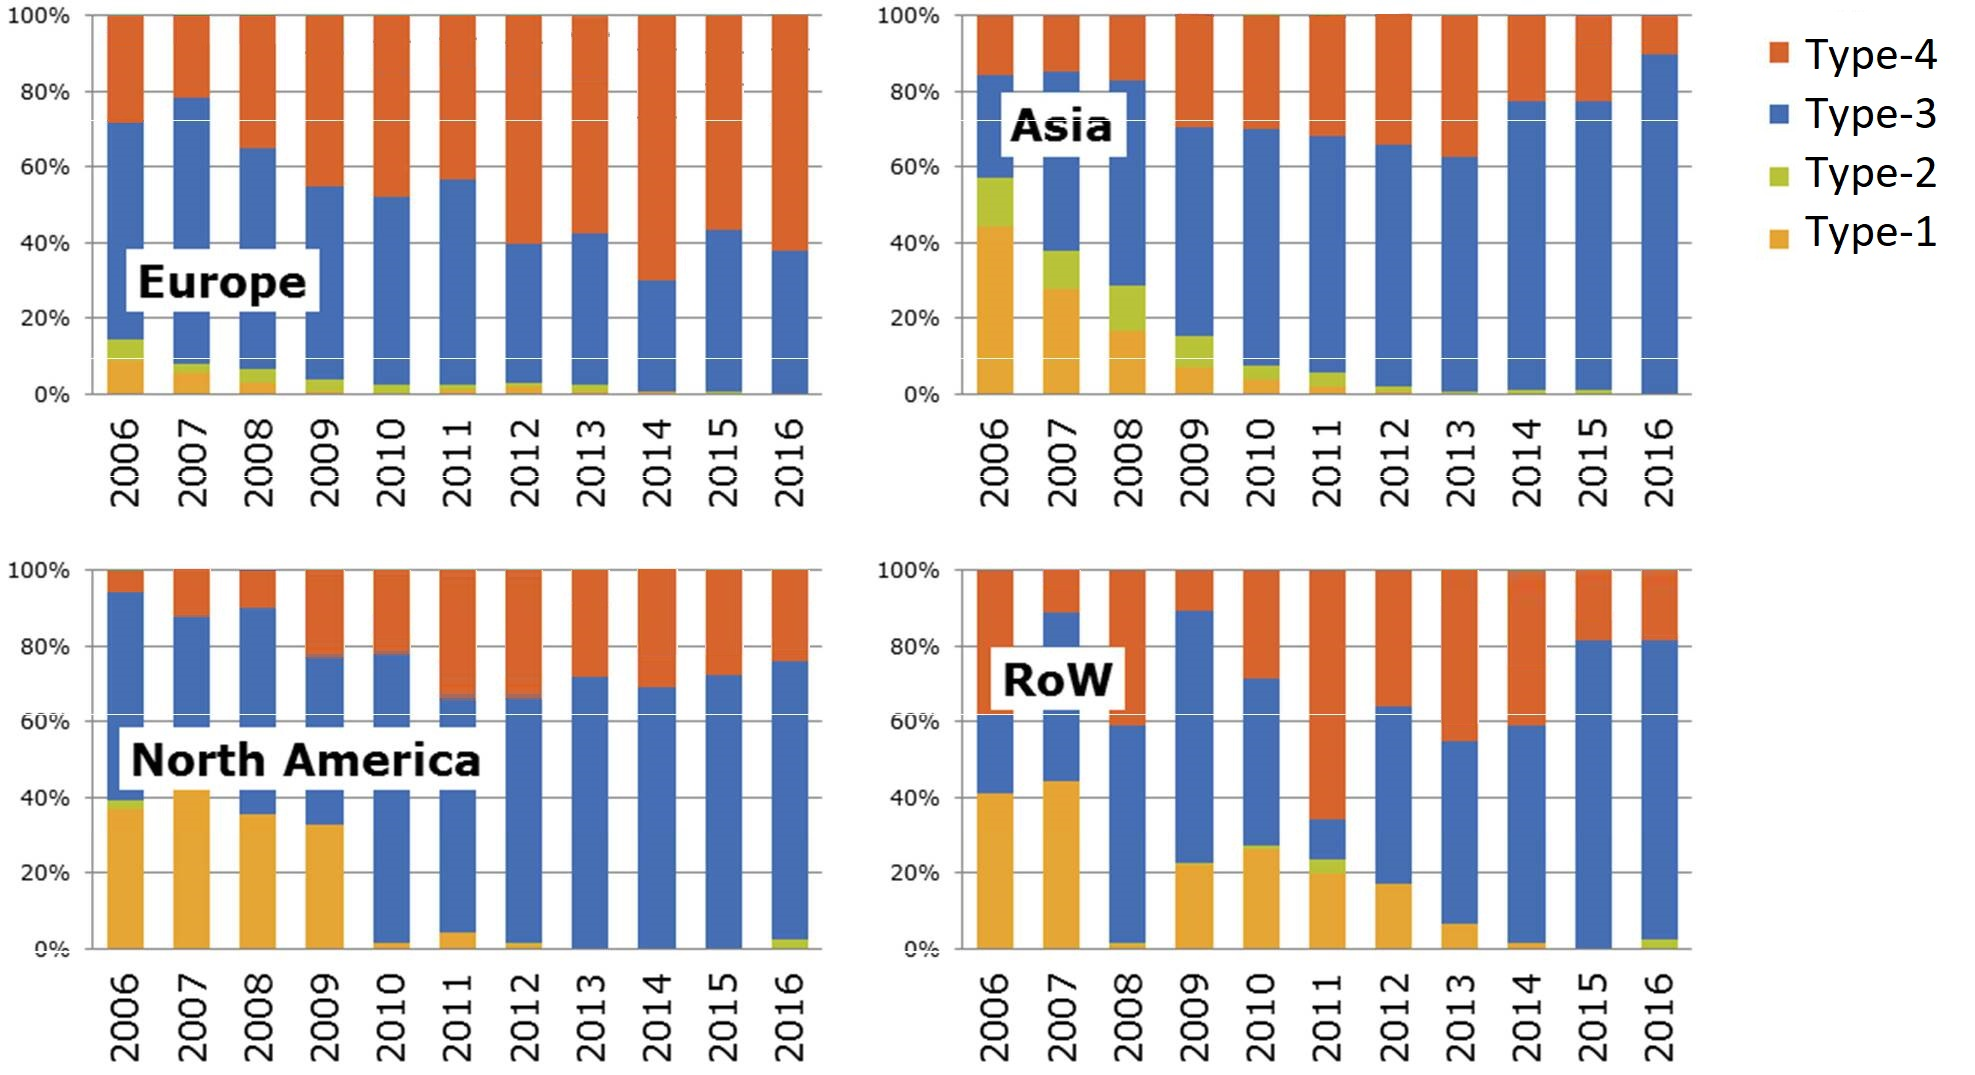
\includegraphics[scale=.2]{Images/WTGTypes.jpg}
	\end{center}
	\legend{Source: JRC}
	\label{fig: WindShare}
\end{figure}

In the light of the data presented above, this work aims to develop a software able to estimate the parameters of a mathematical model capable of predicting the behaviour of Type-3 Wind Turbine Generators. The DFIG mathematical model will be subject to the following chapter. Afterwards, the estimation process and methods will be presented on chapter \ref{ch: Estim}. At last, expected results will be presented on chapter \ref{ch: Res}.

% ---

% ---
% Capítulo 2
% ---
\chapter{Modelling of Wind Turbine Generators}

\label{ch: Mod}

With a growing share of energy covered by wind, system operators must consider how wind turbines affect the system stability during faults and maneuvers. To do so, mathematical models capable of describing these machines' behaviour are crucial. Obtaining these models, on the other hand, is not an easy task, due to considerable amount of wind turbines in large power plants, with different manufacturers, technologies, sizes, distances from point of connection and wind conditions. Thus, a model that describes well a particular turbine in a power plant, won't necessarily work for its neighboring generators. Also, due to industrial secrecy, manufacturers provide little or no information about how their turbines behave. Furthermore, having one model for every wind turbine within a power plant would result in a mathematical problem with high complexity and computational cost \cite{Erlich2012}.

\section{Generic Models of Wind Turbine Generators}

To address this problem, studies such as \cite{Muljadi2008}, \cite{Ellis2011}, \cite{council2008wecc} and \cite{Asmine2011}, motivated specially by the Institute of Electrical and Electronics Engineers (IEEE) and the Western Electricity Coordinating Council (WECC), developed generic models able to predict the behaviour of entire wind power plants. Such models reduced the problem complexity, since they were composed of a single equivalent generator. A two-machine model is needed only in rare cases, such as when the wind power plant is composed of two or more types of wind turbines \cite{Ellis2011}.

These studies have also shown that commercial wind turbine generators (WTG) could be sorted into four basic types, according to its technology \cite{Ellis2011}. These types are described in the following subsections.

\subsection{Type-1: Squirrel Cage Induction Generator}

The first type of wind turbine generator is composed of a Squirrel Cage Induction Generator (SCIG) connected to a wind turbine through a controlled gearbox, as displayed in Figure \ref{fig: WTG1}. Due to its torque-speed characteristics, generators of this type operate at constant rotor speed, requiring robust controllers on gearbox and blade. Besides, as usual to any induction generator, the SCIG absorbs reactive power during operation. Thus, capacitors are often employed for power faction correction purposes. Moreover, type-1 generators limit aerodynamic power by varying the pitch angle of their blades, imposing great mechanical stress on blades, shafts and gears, demanding a robust mechanical design and preventing these generators to operate above certain wind speed \cite{Ellis2011}. 

\begin{figure}[h]
	\caption{Representation of Type-1 Wind Turbine Generator}
	\begin{center}
		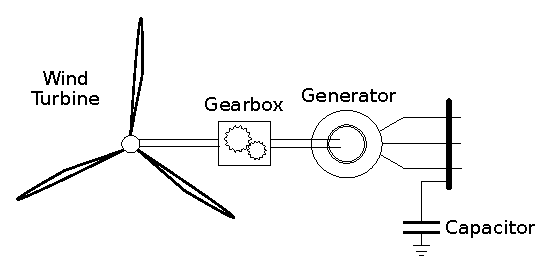
\includegraphics[scale=1]{Images/Type1WTG.eps}
	\end{center}
	\label{fig: WTG1}
\end{figure}

\subsection{Type-2: Wound Rotor Induction Generator}

Similarly to Type-1 WTG, Type-2 Wind Turbine Generators are composed of an asynchronous machine connected to a wind turbine via gearbox, but, instead of SCIG, Wound Rotor Induction Generator (WRIG) are used to convert kinetic energy into electricity. The WRIG has access to its rotor windings, allowing to vary the rotor resistance. As a direct consequence, this machine can operate in different wind speeds by adjusting its torque-speed curve as needed \cite{Ellis2011}. Therefore, Type-2 WTG have a WRIG with a variable resistance connected to its rotor terminals, as shown in Figure \ref{fig: WTG2}.

\begin{figure}[h]
	\caption{Representation of Type-2 Wind Turbine Generator}
	\begin{center}
		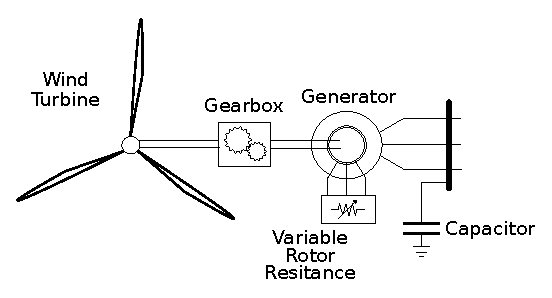
\includegraphics[scale=1]{Images/Type2WTG.eps}
	\end{center}
	\label{fig: WTG2}
\end{figure}

This type of generator has then three speed control systems, with rotor resistance control responding to rapid changes in speed, gearbox control for medium variations and pitch control for slow changes. These control system work together to maintain power output constant and reduce mechanical stress on components. The effects on the torque-speed curve caused by different rotor resistances are shown in Figure \ref{fig: Tw}. For a fixed power, increasing rotor resistance increases the speed needed on the shaft, allowing the wind turbine to operate above rated wind speed. However, the speed range is only $\pm 10\%$ of rated slip. Also, this machine still needs a reactive compensation circuit on its terminals \cite{Muljadi2010}.

\begin{figure}[h]
	\caption{Torque-speed curve}
	\begin{center}
		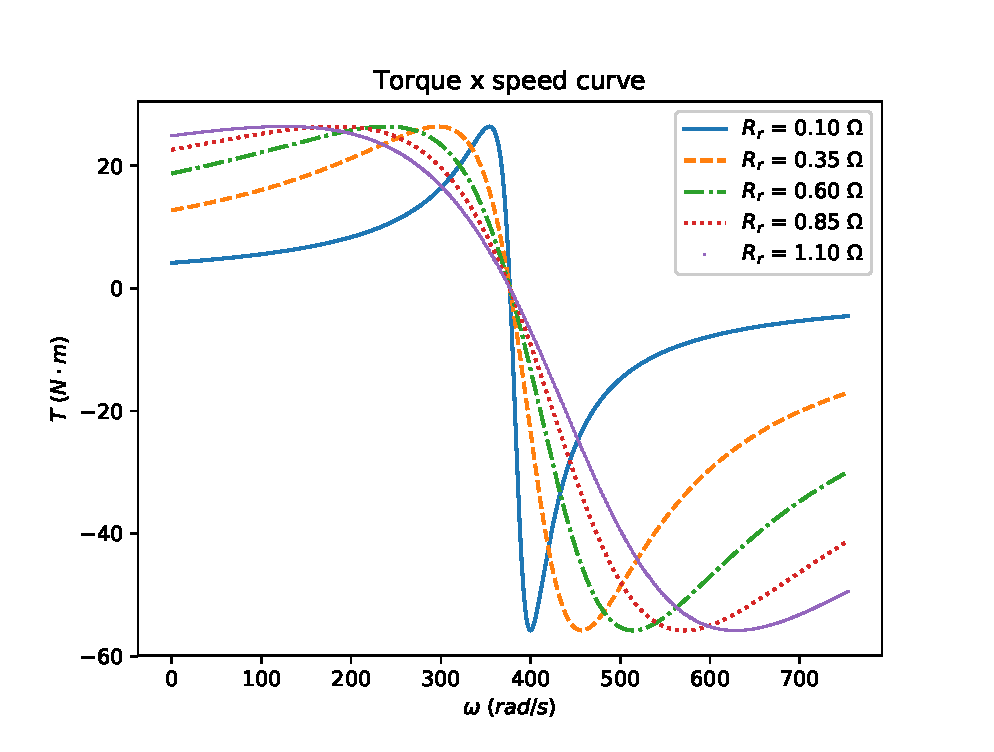
\includegraphics[scale=.7]{Images/Tw_curve.eps}
	\end{center}
	\label{fig: Tw}
\end{figure}

\subsection{Type-3: Doubly Fed Induction Generator}

A Type-3 Wind Turbine Generator, often called Doubly Fed Induction Generator (DFIG), is also composed of a wound rotor machine connected to a wind turbine. But, instead of varying rotor resistance, a DFIG has its rotor supplied with AC voltage by a back-to-back frequency converter, as displayed in Figure \ref{fig: WTG3}. 

\begin{figure}[h]
	\caption{Representation of Type-3 Wind Turbine Generator}
	\begin{center}
		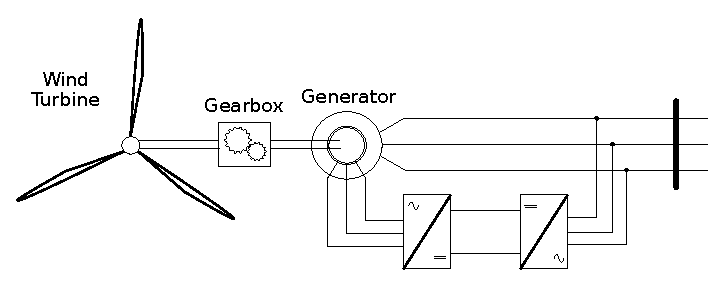
\includegraphics[scale=1]{Images/Type3WTG.eps}
	\end{center}
	\label{fig: WTG3}
\end{figure}

By varying the voltage frequency on the rotor circuit, the generator is able to supply power to the grid in a wider range of wind speed, reaching up to $\pm 30\%$ of rated slip. In addition, the converter can control both real and reactive power independently, ending the necessity of capacitors \cite{Muljadi2010}. Since approximately 30\% of rated power flows through the rotor windings, power electronics components have lower specifications and do not have great impact on overall costs. On the other hand, these generators need regular maintenance due to slip rings, brushes and gearbox, preventing its use in offshore applications \cite{Yaramasu2015}.

\subsection{Type-4: Full-Converter Generator}

The last type of wind turbine generator, also called Full-Converter Generator, is composed of a electrical machine connected to the grid through a back-to-back frequency converter. The converter will operate converting the electrical frequency generated to standard, allowing this type of WTG to operate in a large range of wind speed (up to almost 100\% of rated slip). Due to the converter operation, connection to the wind turbine can be made directly or via gearbox. Likewise, it allows the use of synchronous and asynchronous electrical machines as generator, with Permanent Magnet Synchronous Generator (PMSG), Electrical Excited Synchronous Generator (EESG) and SCIG being most common, because of cost and maintenance purposes. Similar to DFIG, full-converter generators are able to control real and reactive power injected into the grid. However, since all power generated must flow through the power electronics, the overall cost of these generators is usually higher \cite{Yaramasu2015}. Figure \ref{fig: WTG4} depicts a typical Type-4 Wind Turbine Generator.

\begin{figure}[h]
	\caption{Representation of Type-4 Wind Turbine Generator}
	\begin{center}
		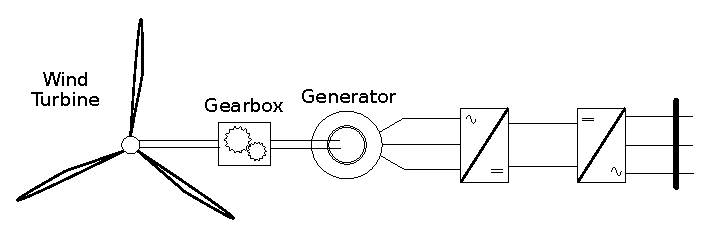
\includegraphics[scale=1]{Images/Type4WTG.eps}
	\end{center}
	\label{fig: WTG4}
\end{figure}

Figure \ref{fig: WindShare} shows the evolution of share in installed capacity onshore for each generator type. The data shows how SCIG and WRIG lost space in the segment and how DFIG and Full-Converter Generators' participation rose, dominating the global market \cite{Magagna2017}.

\begin{figure}[h]
	\caption{Share of installed capacity for each wind turbine generator type}
	\begin{center}
		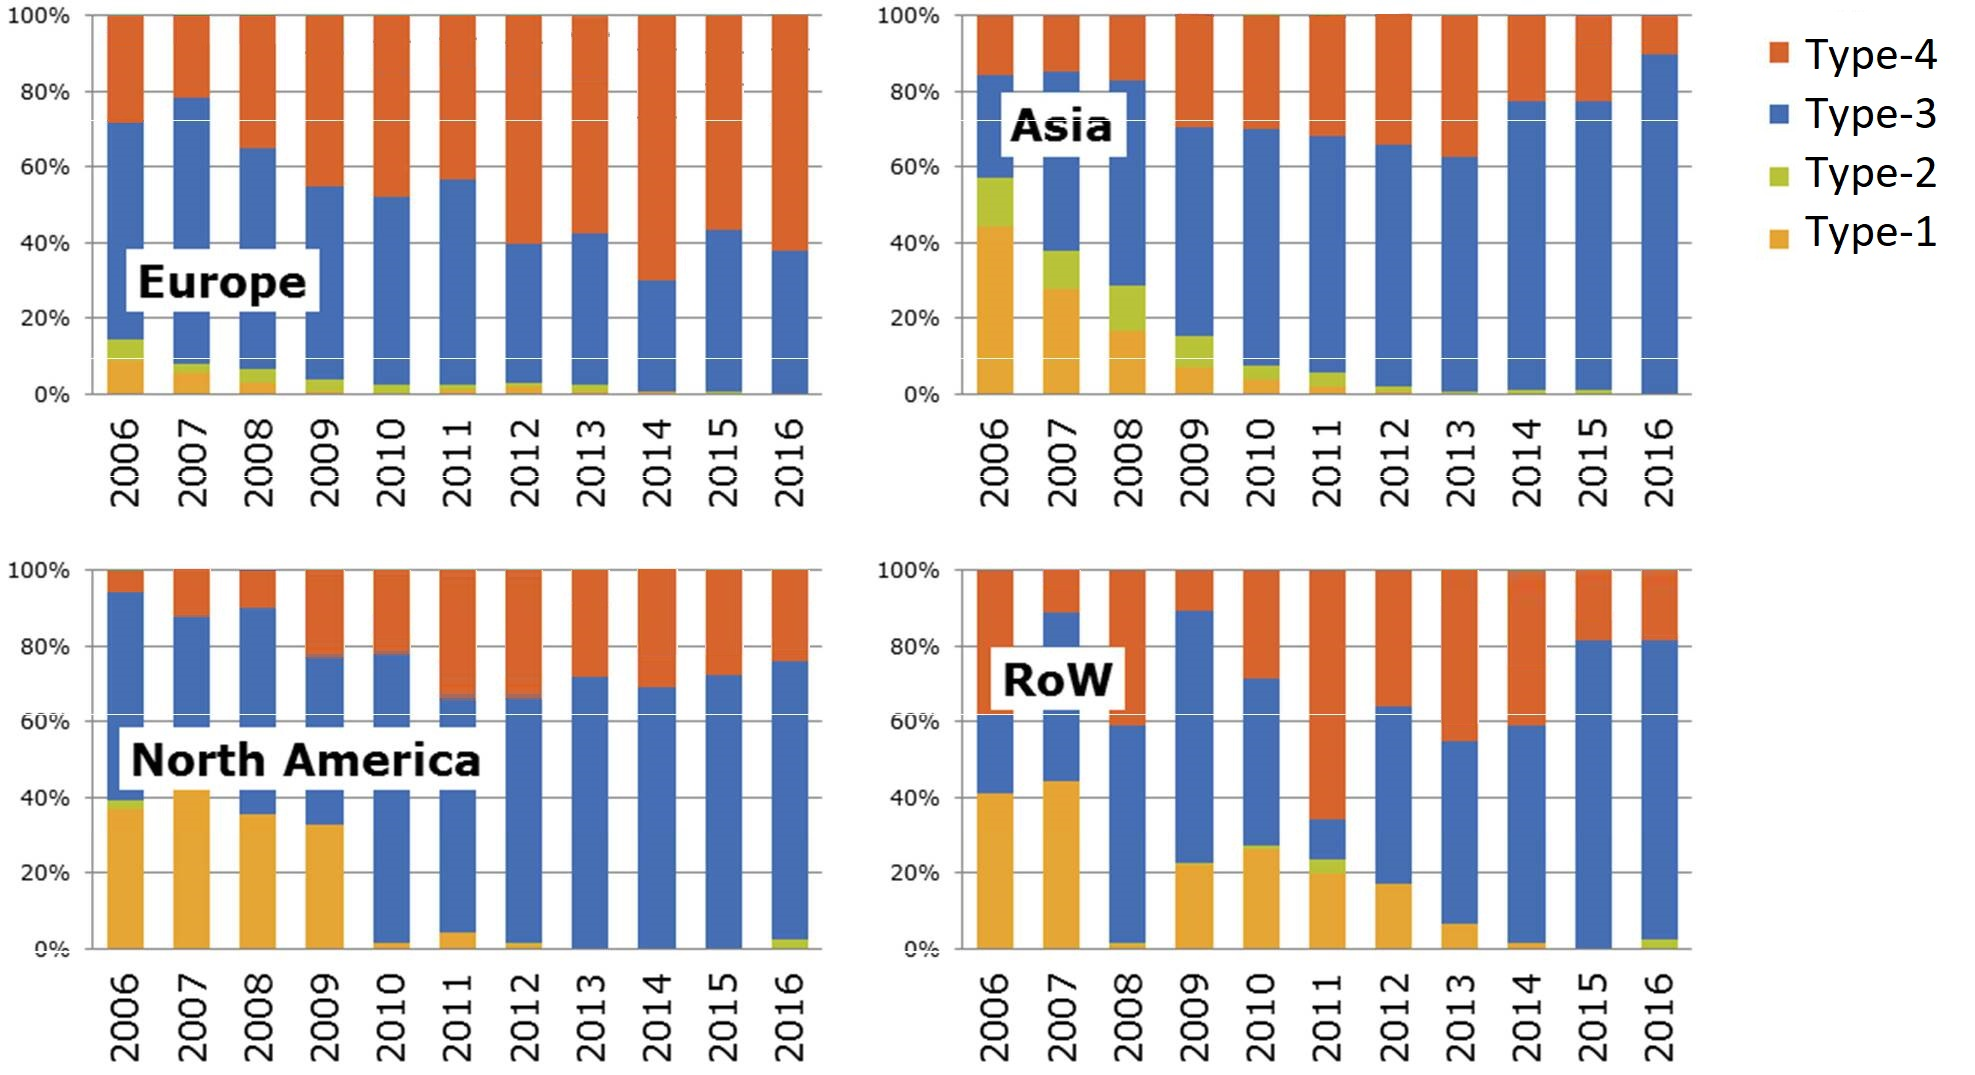
\includegraphics[scale=.2]{Images/WTGTypes.jpg}
	\end{center}
	\legend{Source: JRC}
	\label{fig: WindShare}
\end{figure}

\section{Model of Wind Turbine Generator Selected for Parameter Estimation}

Many mathematical models were developed during the last years that are able to represent Wind Turbine Generators of all types. All those models have in common the fact that they are based on the generic models proposed by the studies made by WECC and IEEE and presented in the last chapter. The mathematical model selected for this work is presented in this section.

Initially proposed by \cite{Erlich2012}, the mathematical model chosen is able to represent the dynamic of both Type-3 and -4 WTG's and can be used to simulate entire wind power plants. In this model, a Thevenin equivalent circuit is connected to grid with a controlled voltage source, as depicted in Figure \ref{fig: ErlMod}. 

\begin{figure}[h]
	\caption{Type-3 WTG model proposed by Erlich}
	\begin{center}
		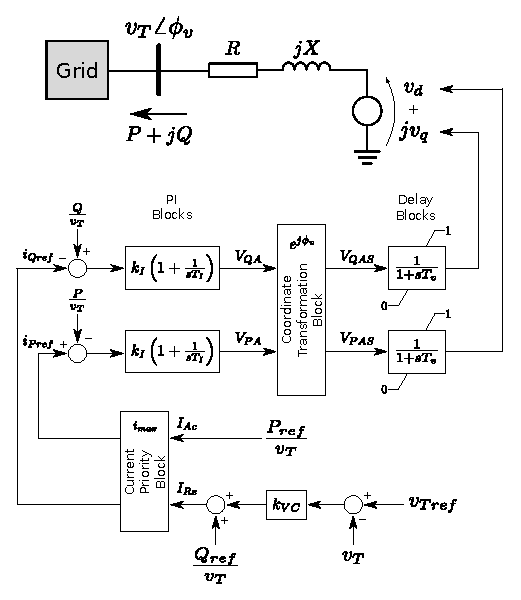
\includegraphics[scale=1]{Images/ErlichModel.eps}
	\end{center}
	\label{fig: ErlMod}
	\legend{Source: Adapted from \cite{Erlich2012}}
\end{figure}

Terminal voltage $v_{T}$ is the variable of interest in this model, appearing as input to DFIG's control system. Active and reactive current are calculated using that input, according to equation \eqref{eq: Currents}.

\begin{equation}
	\begin{cases}
		I_{Ac} = \frac{v_{T}}{p_{Tref}} \\
		I_{Re} = k_{VC}(v_{Tref} - v_{T})
	\end{cases}
	\label{eq: Currents}
\end{equation}

The calculated currents feed a current priority block. This block analyses the current magnitude and terminal voltage level and decides whether power injection or voltage control will be prioritize. In summary, it checks if the generator's current is below a maximum level $i_{max}$ and, if it is not, the block verifies if terminal voltage is above a threshold value $v^{*}$ to decide what will be prioritized. The following algorithm describes the current priority block operation.

\begin{center}
	\begin{lstlisting}[mathescape, columns=fullflexible]
	if $\sqrt{I_{Ac}^{2} + I_{Re}^{2}} \leq i_{max}$ then:
		$\begin{cases}
				i_{Pref} = I_{Ac} \\
				i_{Qref} = I_{Re}
		\end{cases}$
	else:
		if $v_{T} \geq v^{*}$ then:	
			$\begin{cases}
				i_{Pref} = min(i_{max}, I_{Ac}) \\
				i_{Qref} = \sqrt{i_{max}^{2} - i_{Pref}^{2}}
			\end{cases}$
		else:
			$\begin{cases}
				i_{Qref} = min(i_{max}, I_{Re}) \\
				i_{Pref} = \sqrt{i_{max}^{2} - i_{Qref}^{2}}
			\end{cases}$
	\end{lstlisting}
\end{center}

The following PI blocks stand for the DFIG controllers (blade, gearbox, rotor-side and grid-side converters controllers) and their outputs follow the equations presented in \eqref{eq: PI}.

\begin{equation}
	\begin{cases}
		V_{PA} = k_{I}[(i_{Pref} - \frac{p}{v_{T}}) +\frac{1}{T_{I}}\int\displaylimits_{0}^{t}	(i_{Pref} - \frac{p}{v_{T}})dt]\\
		\\
		V_{QA} = k_{I}[(\frac{q}{v_{T}} - i_{Qref}) +\frac{1}{T_{I}}\int\displaylimits_{0}^{t}	(\frac{q}{v_{T}} - i_{Qref})dt]
	\end{cases}
	\label{eq: PI}
\end{equation}

Until here the controller operates on terminal voltage oriented coordinates, so a coordinate transformation block is needed to adequate to synchronous grid coordinates. This block operates according to equations \eqref{eq: CoordShift}.

\begin{equation}
	\begin{cases}
		V_{PAS} = -V_{PA}cos(\theta_{v}) - V_{QA}sin(\theta_{v}) \\
		V_{QAS} = V_{PA}sin(\theta_{v}) - V_{QA}cos(\theta_{v})
	\end{cases}
	\label{eq: CoordShift}
\end{equation}

Finally, two delay blocks supplying the voltage source (one for each component $d$ and $q$) simulate the delay effects of the electrical machine and the back-to-back converter. Their effects are described by \eqref{eq: DelayBlocks}.

\begin{equation}
	\begin{cases}
		\dot{v}_{d} = \frac{1}{T_{V}}(v_{d} - V_{PAS}) \\
		\dot{v}_{q} = \frac{1}{T_{V}}(v_{q} - V_{QAS})
	\end{cases}
	\label{eq: DelayBlocks}
\end{equation}

The outputs of this model are real and reactive power produced by the WTG and their equations are shown below.

\begin{equation}
	\begin{cases}
		P_{e} = \frac{r(v_{Td}v_{d} + v_{Tq}v_{q} - v_{T}^{2}) + x(v_{Tq}v_{d} - v_{Td}v_{q})}{r^{2} + x^{2}} \\
		Q_{e} = \frac{x(v_{Td}v_{d} + v_{Tq}v_{q} - v_{T}^{2}) - r(v_{Tq}v_{d} - v_{Td}v_{q})}{r^{2} + x^{2}}
	\end{cases}
	\label{eq: Outputs}
\end{equation}

Thus, this model can be interpreted as follows:

\begin{equation}
	\begin{cases}
		\dot{x} = f(x, u, y, p) \\
		y = g(x, u, y, p)
	\end{cases}
	\label{eq: xdot}
\end{equation}

\noindent where the state variables $x$, inputs $u$, outputs $y$ and parameters $p$ vectors are described by \eqref{eq: x}, \eqref{eq: u}, \eqref{eq: y} and \eqref{eq: p}, respectively.

\begin{equation}
	x = [v_{d}, v_{q}]^T
	\label{eq: x}
\end{equation}

\begin{equation}
	u = [v_{T}, \theta_{v}, P, Q]^T
	\label{eq: u}
\end{equation}

\begin{equation}
	y = [P_{e}, Q_{e}]^T
	\label{eq: y}
\end{equation}

\begin{equation}
	p = [r, x, k_{I}, T_{I}, T_{V}, k_{VC}]^T
	\label{eq: p}
\end{equation}

In \eqref{eq: p}, the parameters correspond to the stator equivalent resistance $r$ and reactance $x$, PI gain $k_{I}$ and time constant $T_{I}$, delay block time constant $T_{V}$ and voltage block gain $k_{VC}$.
% ---
% Capítulo 3 - Citações
% ---
\chapter{Estimation Process}

\label{ch: Estim}

Parameter estimation problems can be interpreted as optimization problems, where one must find the optimal values of parameters in order to reduce the error between real system and model. During the years, many methods were developed to address this problem, but two approaches have been largely employed to obtain its solution. 

The first approach applies metaheuristics to obtain a sufficiently good solution. These methods are used in a variety of cases, ranging from biological to engineering problems, due to the fact that they are not developed for a specific type of problem. Metaheuristics employ a stochastic search to encounter (near-)optimal solutions within a given region. However, they often take a great amount of time to converge to a solution \cite{Blum2003}. Examples of metaheuristics are Ant Colony Optimization, Differential Evolution, Particle Swarm Optimization and Genetic Algorithm. Applications of this approach in electrical power system cases can be found in \cite{Todorovski2006} and \cite{Yoshida2000}.

The second approach applies analytical methods to find a global/local optimum solution. These methods use equations derived from the problem to locate an optimal solution. Thus, they are problem specific and must be adapted from one case to another. Analytical methods often converge in few iterations, reducing processing time, but are sensitive to initial conditions.

In this work is proposed to combine both approaches, reducing the effects of their disadvantages and improving overall convergence. Mean-Variance Mapping Optimization (MVMO) was the metaheuristic chosen for this problem, alongside Trajectory Sensitivity Method (TS) as analytical method. Both methods will be discussed in the following sections.

The flowchart depicted in Figure \ref{fig: flowchart} illustrates how the proposed method works. At first, a disturbance occurs, resulting in a dynamic response of the real system. The real system's outputs are compared to the model behaviour when the same disturbance is applied to it. The error $J(p)$ is evaluated and while it is greater than a given tolerance $t_{1}$, MVMO algorithm will search for a local solution. Afterwards, the error will eventually drop to a value lower than $t_{1}$, and TS will be used to refine the search to a optimal solution, with error level below $t_{2}$. The error will be evaluated through the Least-Squares Method, given by equation \ref{eq: J(p)}, where $y_{r}$ and $y$ stand for the real system and model outputs.

\begin{equation}
	J(p) = \frac{1}{2}\int\displaylimits_{0}^{T_{0}}(y_{r}(t) - y(t))^{T}(y_{r}(t) - y(t))dt
	\label{eq: J(p)}
\end{equation}

\begin{figure}
	\caption{Flowchart of estimation method}
	\begin{center}
		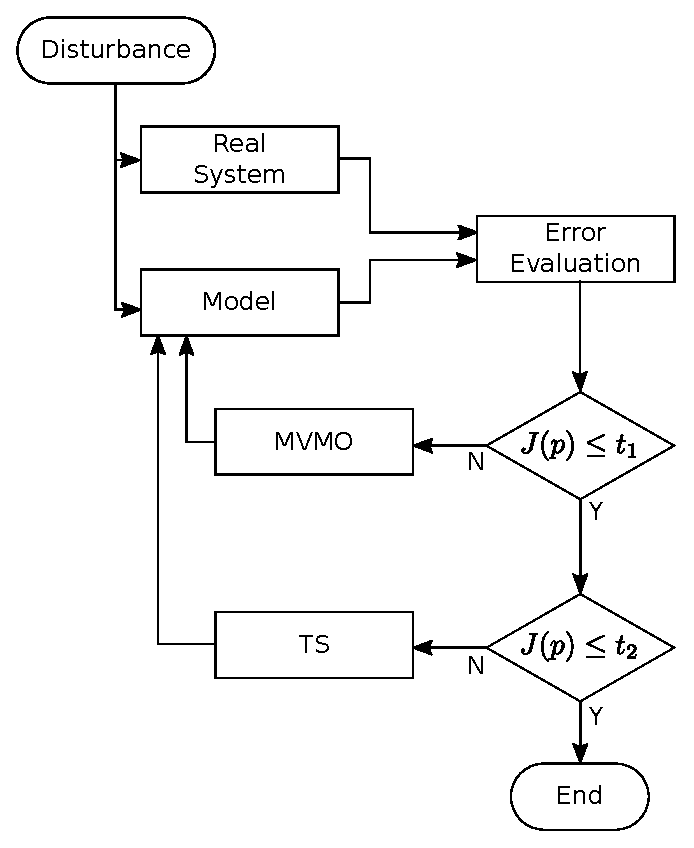
\includegraphics[scale=0.7]{Images/Flowchart.eps}
	\end{center}
	\label{fig: flowchart}
\end{figure}

\section{Mean-Variance Mapping Optimization}

Presented in \cite{Erlich2010}, this population-based metaheuristic shares characteristics with other evolutionary algorithms, but differ from them on how to induce mutations on the offspring in order to diversify the population. By considering statistical data of population during mutation process, MVMO introduces a memory factor to it, enhancing search mechanism. Due this factor, MVMO performs better than similar metaheuristics when population size is relatively small \cite{Nakawiro2011}.

Before the search process starts, a few settings must be done, such as population size, number of offspring, number of genes selected for mutation and selection method. Also, the search region is defined by setting the range within genes can vary. This constrains their values within a feasible region, preventing divergence. The search region is later normalized for all genes, aiding the process. Termination criteria is also set in this step. In this work, both number of generations and fitness will be used as stop criteria.





\section{Trajectory Sensitivity Method}

% ---
% Capítulo 4 - Referencias
% ---
\chapter{Partial Results}

\label{ch: Res}

The expected result of this work is a software capable of correctly estimating the parameters of Type-3 WTG's mathematical model. To do so, the software will apply the proposed estimation method comprises of MVMO and TSM methods combined. 

The measurements will be obtained from a small power system simulated on specific software, such as DIgSILENT or MATLAB. At first, the model proposed in \cite{Erlich2012} will be employed, but it can be further changed if needed. Also, other estimation methods, such as Particle Swarm Optimization, Differential Evolution or Kalman Filters, may be implemented for comparison purposes.

The hybrid approach for parameters estimation presented in this work is already implemented and have shown great results for different models. The approach was used to estimate parameters of simpler systems, such as the spring-mass system, for testing purposes, but also in complex applications, such as load models. The results obtained from those systems are presented in the following subsections.

\section{Results on Spring-Mass System}

The spring-mass system is a simple physical model often used as example of dynamic systems. It is composed of an object of mass $m$ connected to a fixed point in space by a spring of stiffness constant $k$. When disturbed by an external force $u$, the object oscillates and its movement is described on \eqref{eq: SpringMass}, $x$ is the position of the object while $\dot{x}$ and $\ddot{x}$ correspond to its speed and acceleration, respectively.

\begin{equation}
	\begin{bmatrix}
		\dot{x} \\
		\ddot{x}
	\end{bmatrix} = 
	\begin{bmatrix}
		0 & 1 \\
		\frac{k}{m} & 0
	\end{bmatrix}\cdot
	\begin{bmatrix}
		x \\
		\dot{x}
	\end{bmatrix} -
	\begin{bmatrix}
		0 \\
		\frac{1}{m}
	\end{bmatrix}
	\cdot
	u
	\label{eq: SpringMass}
\end{equation}

The behaviour of the real system was obtained through simulation with parameters set at $m = 3\ kg$ and $k = 6\ N/m$. Three different estimation process were executed: TSM isolated, MVMO isolated and the hybrid approach proposed. The tolerance for all three estimations was set at $0.1$.

\subsection{Trajectory Sensitivity Results}

It took only 7 iterations to Trajectory Sensitivity Method estimate the parameters when the initial values were $m_{0} = 7\ kg$ and $k_{0} = 7\ N/m$. This shows how fast this method is when the initial values are in the neighbourhood of the real parameters. Figure \ref{fig: TS_conv} shows the error evolution during estimation suing TSM.

\begin{figure}[h]
	\caption{Error evolution of TSM with $m_{0} = 7\ kg$ and $k_{0} = 7\ N/m$}
	\begin{center}
		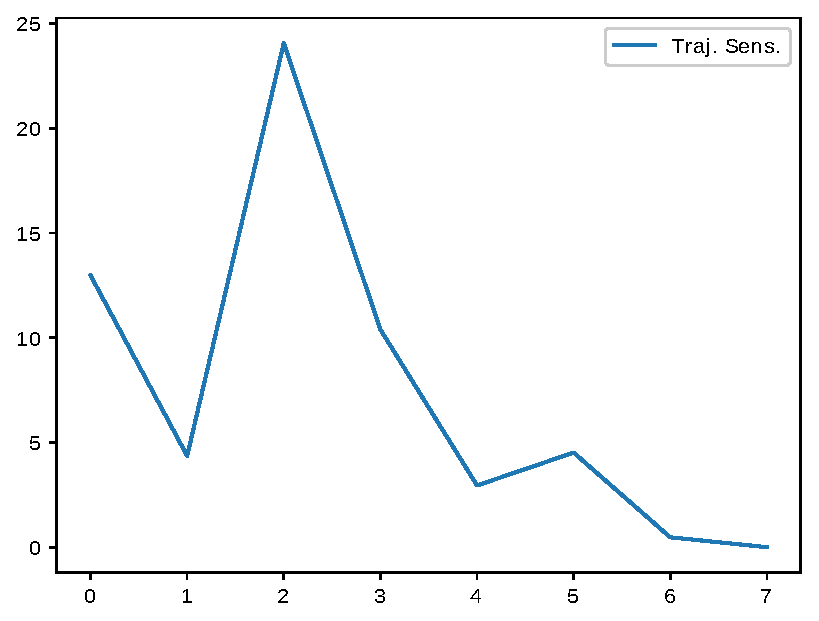
\includegraphics[scale=0.7]{Images/TS_conv.eps}
	\end{center}
	\label{fig: TS_conv}
\end{figure}

However, the convergence region of TSM is extremely limited, diverging from initial points far enough from the real values. The convergence region for the real values was obtained in \cite{Ecyo} and is shown in Figure \ref{fig: conv_reg}. For comparison, the MVMO and the hybrid approach converge for the entire search region displayed on the graph.

\begin{figure}[h]
	\caption{Convergence region of Trajectory Sensitivity Method}
	\begin{center}
		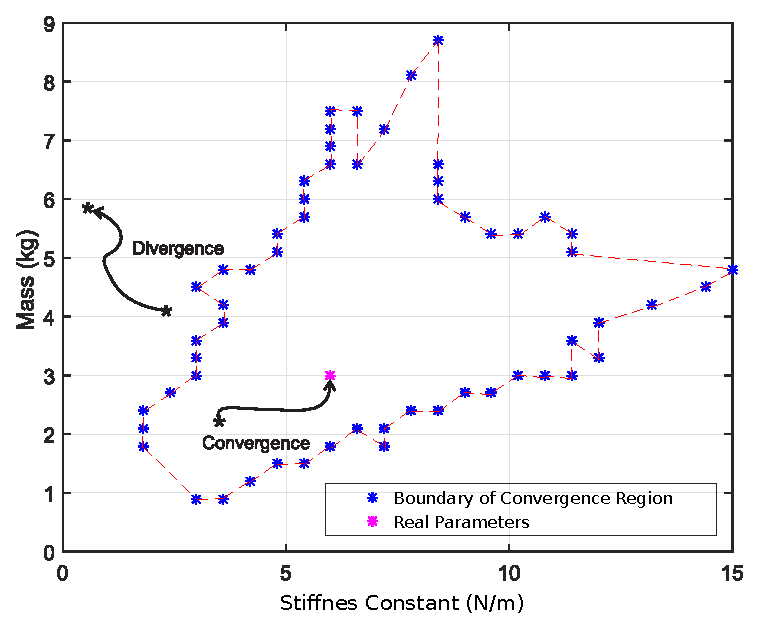
\includegraphics[scale=0.7]{Images/Conv_reg.eps}
	\end{center}
	\label{fig: conv_reg}
	\legend{Source: Adapted from \cite{Ecyo}}
\end{figure}

To illustrate the importance of good initial values, the parameters were reestimated using TSM, but now the initial values were set to be $m_{0} = 8\ kg$ and $k_{0} = 10\ N/m$. Notice that these values are not too far from the ones used in the previous estimation. The results, on the other hand, were extremely different. The method was not able to lower the error below $16.4$ and the parameters found were $m_{f} = 2.7\ kg$ and $k_{f} = 118.6\ N/m$. The error evolution for this estimation is depict in Figure \ref{fig: TS_nconv}.

\begin{figure}[h]
	\caption{Error evolution of TSM with $m_{0} = 8\ kg$ and $k_{0} = 10\ N/m$}
	\begin{center}
		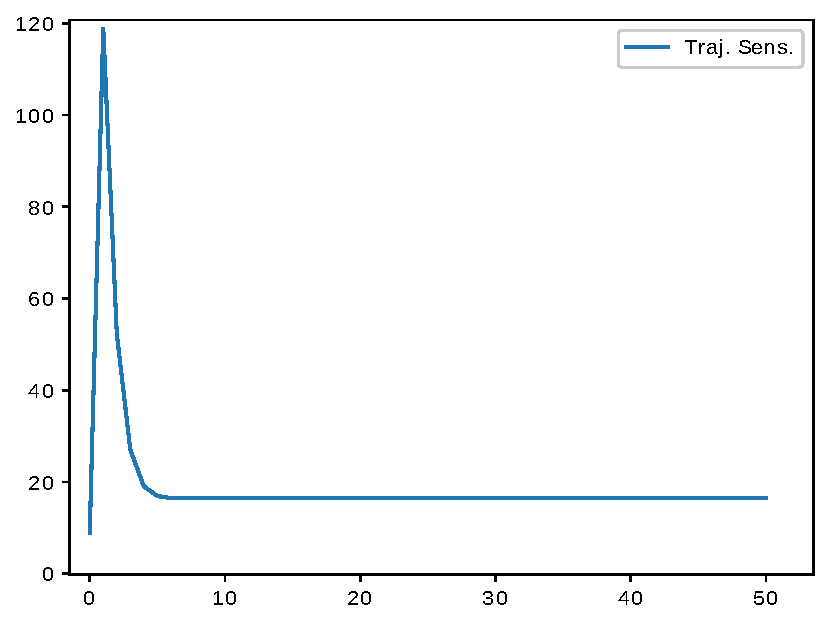
\includegraphics[scale=0.7]{Images/TS_nconv.eps}
	\end{center}
	\label{fig: TS_nconv}
\end{figure}

\subsection{MVMO Results}

The MVMO search region was defined as $0 \leq m \leq 9$ and $0 \leq k \leq 15$. The heuristic method converged after almost 10000 generations, as depicted in Figure \ref{fig: MVMO_conv}. This figure also shows how MVMO rapidly reduces error of estimation, but as the values approach the neighbourhood of the real values, it slows down.

\begin{figure}[h]
	\caption{Error evolution of MVMO}
	\begin{center}
		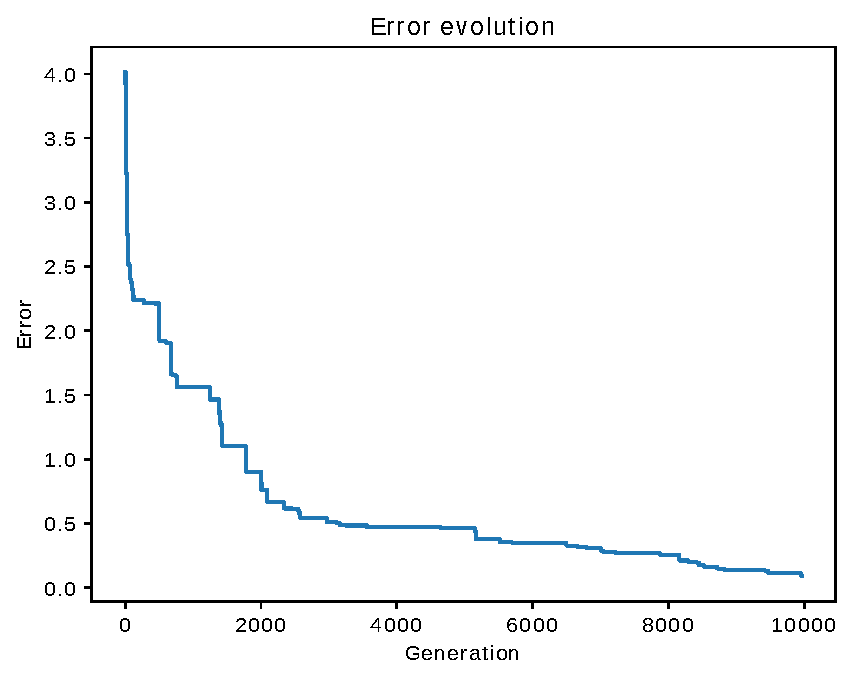
\includegraphics[scale=0.7]{Images/MVMO_conv.eps}
	\end{center}
	\label{fig: MVMO_conv}
\end{figure}

\subsection{Hybrid Approach Results}

By combining both methods, the hybrid approach benefits from the quick error reduction provided by MVMO and the fast convergence from TSM when inside convergence region. The error evolution obtained from this approach is depicted in Figure \ref{fig: Hybrid_conv}

\begin{figure}[h]
	\caption{Results of hybrid approach for spring-mass system}
	\begin{center}
		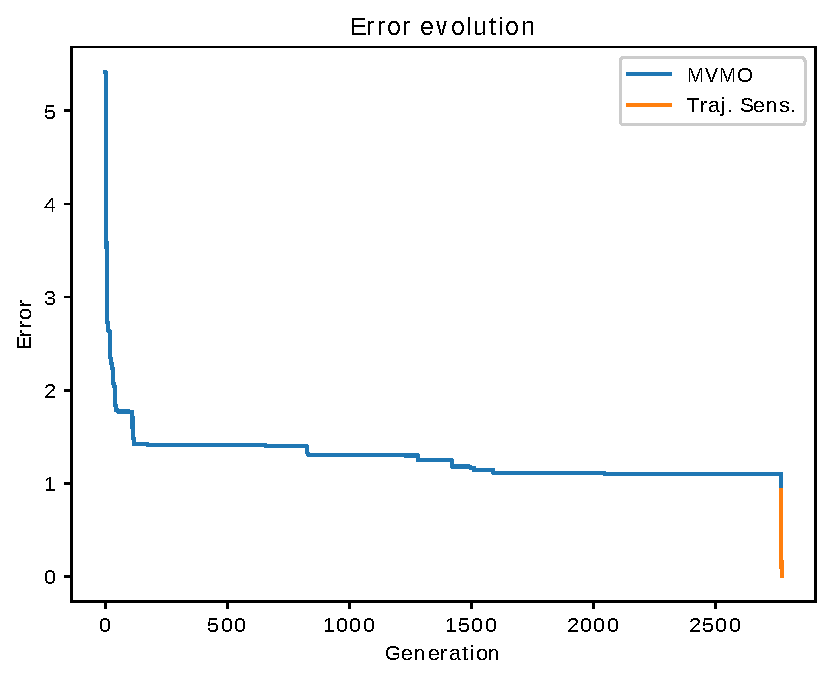
\includegraphics[scale=0.7]{Images/Hybrid_conv.eps}
	\end{center}
	\label{fig: Hybrid_conv}
\end{figure}

When compared to the methods alone, the hybrid approach converges faster than MVMO but slower than TSM, as shown in Table \ref{tab: SM}. Although all methods converged parameters with error level below the tolerance, TSM and the Hybrid approach provided a better behaviour than MVMO with final error close to $2.0\times 10^{-3}$.

\begin{table}[h]
	\caption{Comparison of approaches}
	\begin{center}
	\begin{tabular}{c|c|c}
		Approach & Time & Final Error \\
		\hline
		TSM  & $7 \ s$  & $2.76\times 10^{-3}$ \\
		MVMO  & $10 \ min$  & $89.33\times 10^{-3}$\\
		Hybrid  & $24 \ min$  & $1.54\times 10^{-3}$
	\end{tabular}
	\end{center}
	\label{tab: SM}
\end{table}

\section{Results on Z-IM Load Model}

The hybrid approach was also employed on parameter estimation of Z-IM load model and is subject of a paper presented by the author on the 2019 IEEE Canadian Conference on Electrical and Computer Engineering. This model is able to predict the behaviour of electrical loads during faults in the grid. It is described by the following equations:

\begin{equation}
    \begin{cases}
        \dot{E'} = \frac{1}{T_o}\left(\frac{X}{X'}E' + \frac{X - X'}{X'}V\cos\delta\right) \\
        \dot{\delta} = \omega - \omega_s - \frac{X - X'}{X'}.\frac{V\sin\delta}{T_o E'} \\
        \dot{\omega} = \frac{1}{M}\left(-\frac{VE'\sin\delta}{X'} - T_m\right)
    \end{cases}
    \label{eq: xZIM}
\end{equation}

Its outputs are the active and reactive power consumed by the load and are given by:

\begin{equation}
    \begin{cases}
        P = G_sV^2 - \left(\frac{VE'}{X'}\right)\sin\delta \\
        Q = B_sV^2 + \frac{V(V - E'\cos\delta)}{X'}
    \end{cases}
    \label{eq: yZIM}
\end{equation}

The Z-IM load model is much more complex than the spring-mass system, with 9 parameters to be estimated. The hybrid approach proposed was able to estimate the parameters of this system and the comparison between real and modeled behaviour with the parameters obtained can be seen in the Figure \ref{fig: ZIM}.

\begin{figure}[h]
	\caption{Result of parameter estimation for Z-IM Load Model}
	\begin{center}
		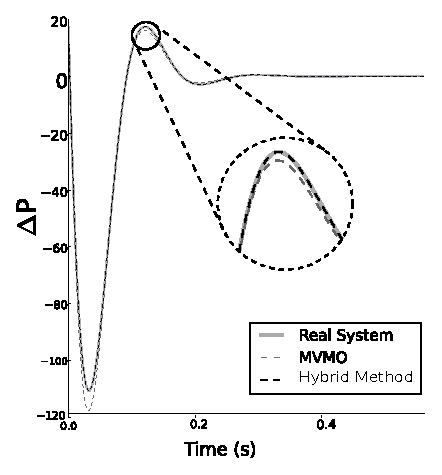
\includegraphics[scale=1]{Images/ZIM.eps}
	\end{center}
	\label{fig: ZIM}
	\legend{Source: \cite{Gomes2019}}
\end{figure}

\section{Ongoing Progress}

With the methods already implemented and tested, the focus is now on the DFIG model. The model has presented some results, but it is not as accurate as expected, requiring some studies about this topic. The implementation of other WTG models for comparison is also under study.

The simulation of wind turbine generators and power plants on specific software will be carried out on the next months. The GUI is under development and already has some features implemented using Python's library \textit{Tkinter}. A proposal to also develop features using \textit{Qt}, a different GUI tool package, is currently under consideration.
% ---

% Capítulo 5 - Conclusão
% ---
%% USPSC-Cap3-Conclusao.tex
% Capítulo 3 - Conclusão
% ---
% Conclusão
% ---
\chapter{Conclusão}
% ---
% O comando abaixo insere parágrafos aleatórios só para exemplificar
Apresentar as conclusões correspondentes aos objetivos ou hipóteses propostos para o desenvolvimento do trabalho, podendo incluir  sugestões para novas pesquisas.

O Grupo desenvolvedor do Pacote USPSC, atualmente na versão 2.0 composta pela \textbf{Classe USPSC}, pelo \textbf{Modelo para TCC em \LaTeX\ utilizando a classe USPSC} e pelo \textbf{Modelo para teses e dissertações em \LaTeX\ utilizando a classe USPSC}, acredita que esta ferramenta propiciará o aprimoramento na qualidade dos trabalhos acadêmicos produzidos pelos alunos de pós-graduação das Unidades de Ensino e Pesquisa do Campus USP de São Carlos, garantindo a normalização e padronização estabelecidas.

O Modelo para TCC está disponível inicialmente apenas para EESC, em conformidade com a \textbf{ABNT NBR 14724}: informação e documentação: trabalhos acadêmicos: apresentação \cite{nbr14724}, \textbf{Diretrizes para apresentação de dissertações e teses da USP}: documento eletrônico e impresso - Parte I (ABNT) \cite{sibi2016} e as \textbf{Diretrizes para elaboração de trabalhos acadêmicos nas EESC-USP} \cite{eesc2016}. Será estendido às demais Unidades de Ensino do Campus USP de São Carlos a medida que as mesmas definirem seus padrões. 


O Grupo desenvolvedor do Pacote USPSC já está trabalhando para que a Classe USPSC seja uma  customização em conformidade com as orientações dadas em \url{https://github.com/abntex/abntex2/wiki/ComoCustomizar}.

A expectativa é de que tais soluções sejam adotadas por outras Unidades da USP e outras instituições interessadas, sendo que a facilidade de customização fatalmente contribuirá para tanto.


% ---

% ----------------------------------------------------------
% ELEMENTOS PÓS-TEXTUAIS
% ----------------------------------------------------------
\postextual
% ----------------------------------------------------------

% -----------------------------------------------------------
% Referências bibliográficas
% ----------------------------------------------------------
\bibliography{USPSC-modelo-references}


% ----------------------------------------------------------
% Glossário
% ----------------------------------------------------------
%
% Consulte o manual da classe abntex2 para orientações sobre o glossário.
%
%\glossary

% ----------------------------------------------------------
% Apêndices
% ----------------------------------------------------------
%% USPSC-Apendice.tex
% ---
% Inicia os apêndices
% ---

\begin{apendicesenv}
% Imprime uma página indicando o início dos apêndices
\partapendices

\chapter{Parameter Estimation of Spring-Mass Model}

The spring-mass system is a simple physical model often used as example of dynamic systems. It is composed of an object of mass $m$ connected to a fixed point in space by a spring of stiffness constant $k$. When disturbed by an external force $u$, the object oscillates and its movement is described by \eqref{eq: SpringMass}, $x$ is the position of the object while $x_{1}$ and $x_{2}$ correspond to its speed and acceleration, respectively. The system output, parameter vector, input and initial conditions are presented on \eqref{eq: SMoutput}, \eqref{eq: SMp}, \eqref{eq: SMinput} and \eqref{eq: SMinitcond}, respectively.

\begin{equation}
	\begin{bmatrix}
		\dot{x_{1}} \\
		\dot{x_{2}}
	\end{bmatrix} = 
	\begin{bmatrix}
		0 & 1 \\
		\frac{k}{m} & 0
	\end{bmatrix}\cdot
	\begin{bmatrix}
		x_{1} \\
		x_{2}
	\end{bmatrix} -
	\begin{bmatrix}
		0 \\
		\frac{1}{m}
	\end{bmatrix}
	\cdot
	u
	\label{eq: SpringMass}
\end{equation}

\begin{equation}
	y = \begin{bmatrix}
		x_{1}, x_{2}
	\end{bmatrix}^ {T}
	\label{eq: SMoutput}
\end{equation}

\begin{equation}
	p = \begin{bmatrix}
		m, k
	\end{bmatrix}^ {T}
	\label{eq: SMp}
\end{equation}

\begin{equation}
	u(t = 0) = 1
	\label{eq: SMinput}
\end{equation}

\begin{equation}
	\begin{cases}
		x_{1}(0) = 0 \\
		x_{2}(0) = 0
	\end{cases}
	\label{eq: SMinitcond}
\end{equation}

The behaviour of the real system was obtained by means of simulation with parameters set at $m = 3\ kg$ and $k = 6\ N/m$. Three different estimation process were executed: TSM, MVMO and the hybrid approach of MVMO and TSM combined. The tolerance for all three estimations was set at $tol = 0.1$.

\section{Trajectory Sensitivity Results}

It took only 7 iterations (7 seconds on a PC) for Trajectory Sensitivity Method to estimate the parameters when the initial values were $m_{0} = 7\ kg$ and $k_{0} = 7\ N/m$. This shows how fast this method is, as long as the initial values are in the neighbourhood of the real parameters. Figure \ref{fig: TS_conv} shows the error evolution during estimation suing TSM.

\begin{figure}[h]
	\caption{Error evolution of TSM with $m_{0} = 7\ kg$ and $k_{0} = 7\ N/m$}
	\begin{center}
		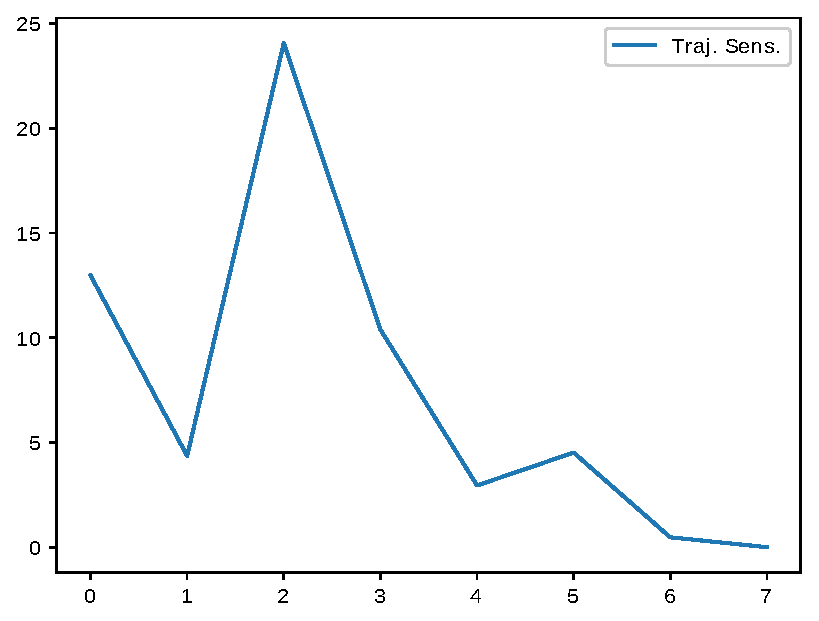
\includegraphics[scale=0.7]{Images/TS_conv.eps}
	\end{center}
	\label{fig: TS_conv}
\end{figure}

However, the convergence region \footnote{Convergence region is a region in parameter space where, if the initial guess for parameter values is inside it, the convergence to true values is guaranteed.} of TSM is extremely limited, diverging for initial points far enough from the real values. The convergence region for the real values was obtained in \cite{Ecyo} and is shown in Figure \ref{fig: conv_reg}. For comparison, the MVMO and the hybrid approach converge for the entire search region displayed on the graph.

\begin{figure}[h]
	\caption{Convergence region of Trajectory Sensitivity Method}
	\begin{center}
		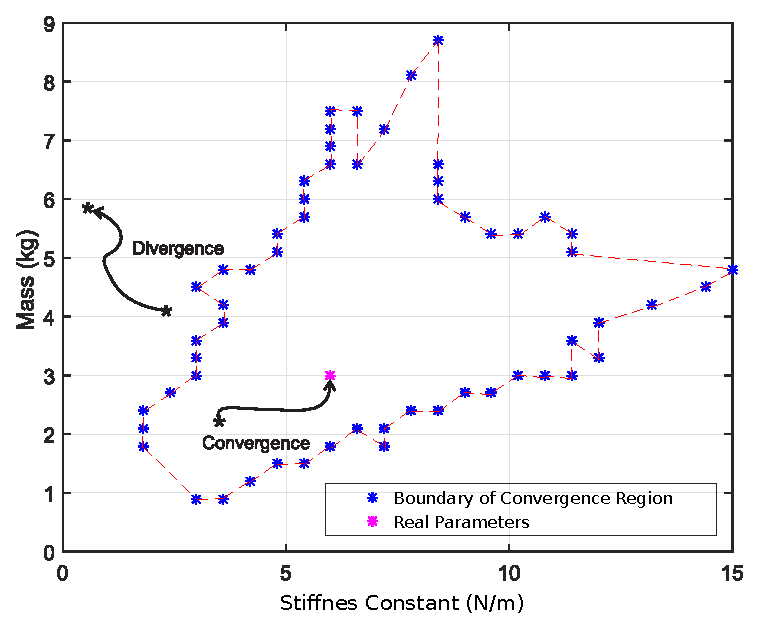
\includegraphics[scale=0.7]{Images/Conv_reg.eps}
	\end{center}
	\label{fig: conv_reg}
	\legend{Source: Adapted from \cite{Ecyo}}
\end{figure}

To illustrate the importance of good initial values, the parameters were reestimated using TSM, but now the initial values were set to be $m_{0} = 8\ kg$ and $k_{0} = 10\ N/m$. Notice that these values are not too far from the ones used in the previous estimation. The results, on the other hand, were extremely different. The method was not able to lower the error below $16.4$ and the parameters found were $m_{f} = 2.7\ kg$ and $k_{f} = 118.6\ N/m$. The error evolution for this estimation is depict in Figure \ref{fig: TS_nconv}.

\begin{figure}[h]
	\caption{Error evolution of TSM with $m_{0} = 8\ kg$ and $k_{0} = 10\ N/m$}
	\begin{center}
		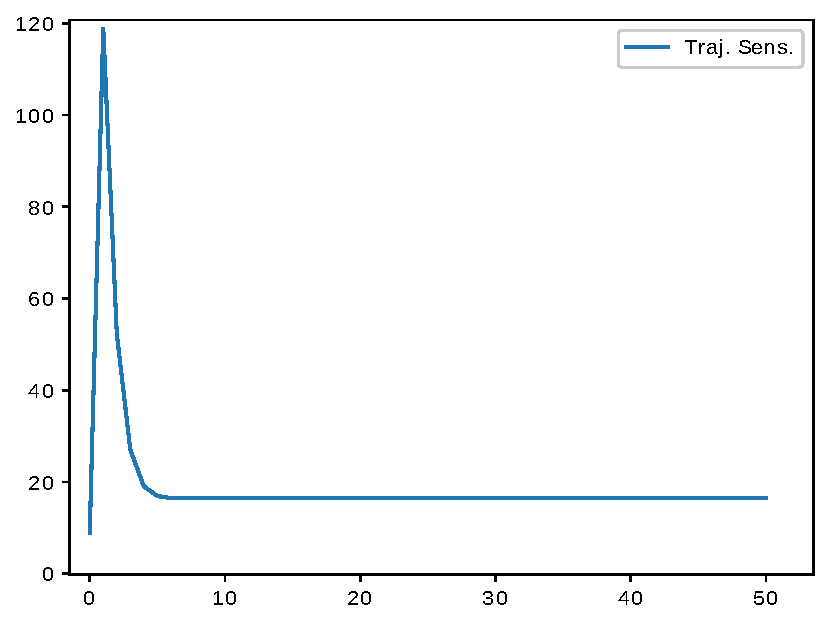
\includegraphics[scale=0.7]{Images/TS_nconv.eps}
	\end{center}
	\label{fig: TS_nconv}
\end{figure}

\section{MVMO Results}

To use MVMO, a search region in parameter space must be defined. Therefore, the parameters boundaries was defined as $0 \leq m \leq 9$ and $0 \leq k \leq 15$. The population size was set at 5 individuals and after every generation 1 new individual was created. The heuristic method converged after almost 10000 generations, as depicted in Figure \ref{fig: MVMO_conv}. This figure also shows how MVMO rapidly reduces error of estimation, but as the values approach the neighbourhood of the real values, it slows down.

\begin{figure}[h]
	\caption{Error evolution of MVMO}
	\begin{center}
		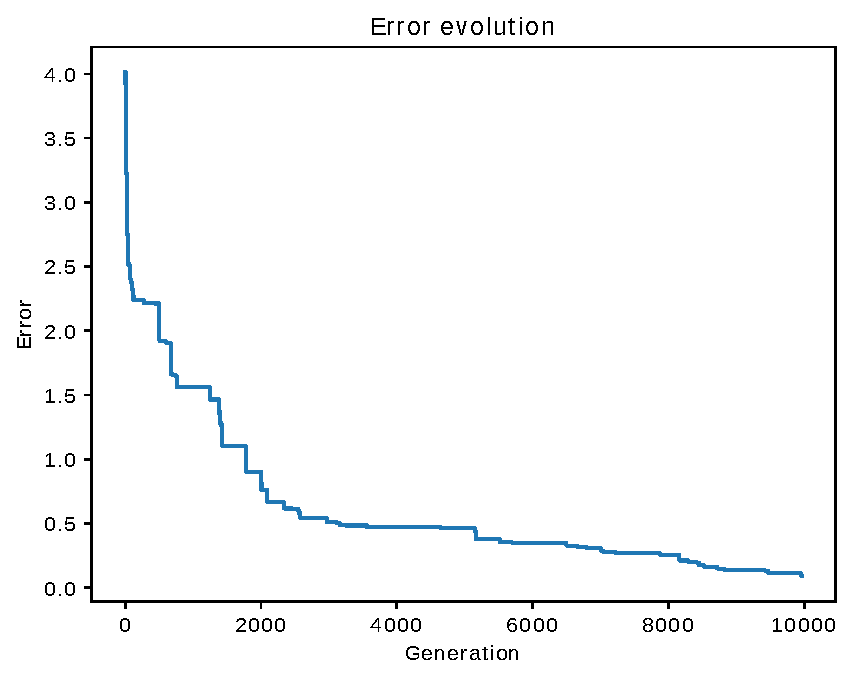
\includegraphics[scale=0.7]{Images/MVMO_conv.eps}
	\end{center}
	\label{fig: MVMO_conv}
\end{figure}

\section{Hybrid Approach Results}

By combining both methods, the hybrid approach benefits from the quick error reduction provided by MVMO and the fast convergence from TSM when inside convergence region. The error evolution obtained from this approach is depicted in Figure \ref{fig: Hybrid_conv}. The tolerance for this approach were set at $tol_{1} = 1.5$ and $tol_{2} = 0.1$.

\begin{figure}[h]
	\caption{Results of hybrid approach for spring-mass system}
	\begin{center}
		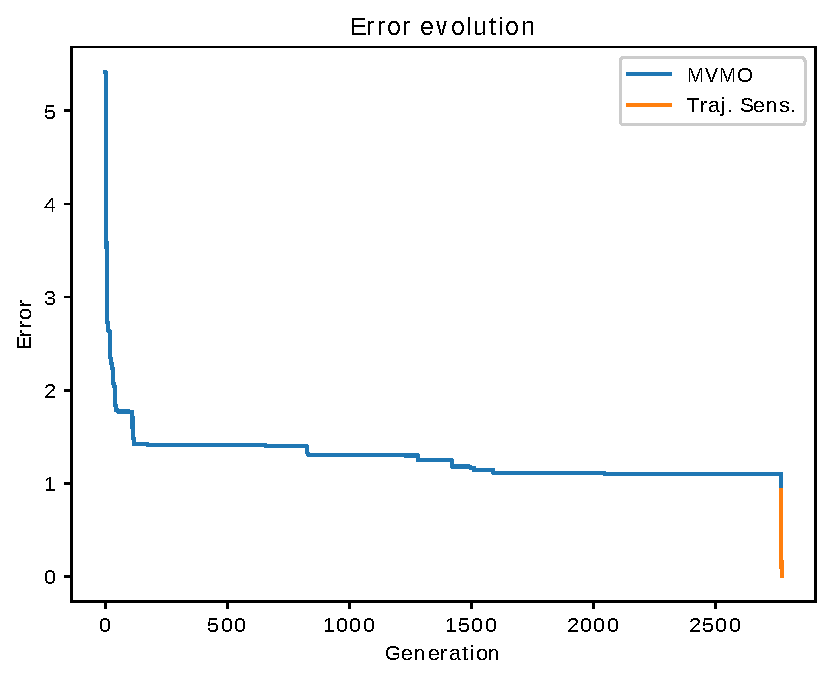
\includegraphics[scale=0.7]{Images/Hybrid_conv.eps}
	\end{center}
	\label{fig: Hybrid_conv}
\end{figure}

When compared to each method, the hybrid approach converges faster than MVMO but slower than TSM, as shown in Table \ref{tab: SM}. Although all methods converged to parameter values that resulted in an error level below the tolerance, TSM and the Hybrid approach provided final results with error level below the values obtained by MVMO.

\begin{table}[h]
	\caption{Comparison of approaches}
	\begin{center}
	\begin{tabular}{c|c|c}
		Approach & Time & Final Error \\
		\hline
		TSM  & $7 \ s$  & $2.76\times 10^{-3}$ \\
		MVMO  & $24 \ min$  & $89.33\times 10^{-3}$\\
		Hybrid  & $10 \ min$  & $1.54\times 10^{-3}$
	\end{tabular}
	\end{center}
	\label{tab: SM}
\end{table}

%------------------------------------------------------------
\chapter{Parameter Estimation of Linearized Z-IM Load Model}

The hybrid approach was also employed on parameter estimation of Z-IM Load Model. This model is able to predict the behaviour of electrical loads during faults in the grid. The Z-IM Load Model is composed of an impedance in parallel with a third-order induction motor (IM), as shown in Figure \ref{img: Z-IM}. According to \cite{Choi}, this model results in low error levels for both active and reactive power, alongside having a smaller parameter vector when compared with other models. It is described by the following equations:

\begin{figure}[h]
    \caption{Schematic of Z-IM Load Model.}
    \begin{center}
    	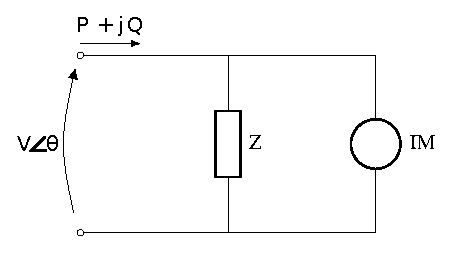
\includegraphics[scale=1]{Images/drawZIM.eps}
    \end{center}
    \label{img: Z-IM}
\end{figure}

\begin{equation}
    \begin{cases}
        \dot{\Delta E'} = \frac{-1}{T_{o}X'}[X\Delta E' + (X - X')V_{0}\sin\delta_{0}\Delta \delta] + \frac{(X - X')\cos\delta_{0}}{T_{0}X'}\Delta V \\
        \\
        \dot{\Delta \delta} = \frac{(X-X')V_{0}}{T_{0}X'E'_{0}}\cdot\left(\frac{\sin\delta_{0}\Delta E'}{E'_0} - \cos\delta_{0}\Delta\delta\right) + \Delta\omega - \frac{(X - X')\sin\delta_0}{T_o X'E'_0}\Delta V \\
        \\
        \dot{\Delta \omega} = \frac{-V_{0}}{MX'}(\sin\delta_{0}\Delta E' + E'_{0}\cos\delta_{0}\Delta\delta) - \frac{E'_0\sin\delta_0}{MX'}\Delta V
    \end{cases}
    \label{eq: xZIM}
\end{equation}

\begin{equation}
    \begin{cases}
        \Delta P = \frac{-V_{0}}{X'}(\sin{\delta_{0}}\Delta E' + E'_{0}\cos{\delta_{0}}\Delta \delta) + \left(2G_{s} V_{0} - \frac{E'_{0} \sin{\delta_{0}}}{X'}\right)\Delta V \\
        \\
        \Delta Q = \frac{-V_{0}}{X'}(\cos{\delta_{0}}\Delta E' + E'_{0}\sin{\delta_{0}}\Delta\delta) + \left(2B_{s} V_{0} + \frac{2V_{0} - E'_{0} \cos{\delta_{0}}}{X'}\right)\Delta V
    \end{cases}
    \label{eq: yZIM}
\end{equation}

\begin{equation}
    \begin{cases}
    X = X_{s} + X_{m} \\
    X' = X_{s} + \frac{X_{m} X_{r}}{X_{m} + X_{s}} \\
    T_{o} = \frac{X_{r} + X_{m}}{\omega_{s} R_{r}}
    \end{cases}
    \label{eq: terms}
\end{equation}

\noindent where the terms $\Delta E'$ and $\Delta \delta$ represent the variation on voltage magnitude and angle at the motor terminals, $\Delta \omega$ is the variation on stator speed, in rad/s. $X_m$, $X_s$ and $X_r$ are the magnetizing, stator and rotor reactances, respectively, $R_r$ stands for the rotor resistance, $\omega_{s}$ is the synchronous speed, $T_o$ represents the open-circuit transient time constant, $M$ is the motor inertia and $V_{0}$ is the voltage on the load terminals before the disturbance. The state, output, input and parameter vectors are presented in \eqref{eq: ZIMstate}, \eqref{eq: ZIMoutput}, \eqref{eq: ZIMinput} and \eqref{eq: ZIMparam}, respectively.

\begin{equation}
	x = [\Delta E', \Delta \delta, \Delta \omega]^{T}
	\label{eq: ZIMstate}
\end{equation}

\begin{equation}
	y = [\Delta P, \Delta Q]^{T}
	\label{eq: ZIMoutput}
\end{equation}

\begin{equation}
	u = [\Delta V]
	\label{eq: ZIMinput}
\end{equation}

\begin{equation}
	p = [X, X', T_{0}, M, G_{s}, B_{s}, E'_{0}, \delta_{0}]^{T}
	\label{eq: ZIMparam}
\end{equation}

The Z-IM load model is much more complex than the spring-mass system, with 9 parameters to be estimated. The hybrid approach proposed was able to estimate the parameters of this system and the comparison between real and modeled behaviour with the parameters obtained can be seen in the Figure \ref{fig: ZIM}.

\begin{figure}[h]
	\caption{Result of parameter estimation for Z-IM Load Model}
	\begin{center}
		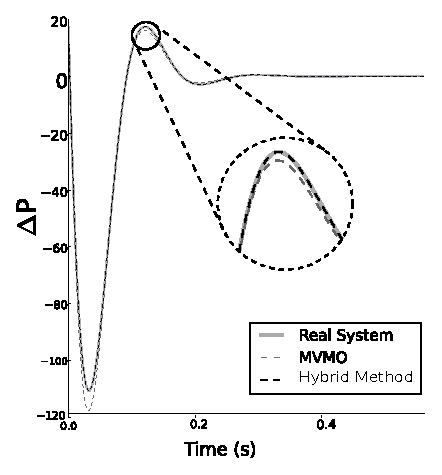
\includegraphics[scale=1]{Images/ZIM.eps}
	\end{center}
	\label{fig: ZIM}
	\legend{Source: \cite{Gomes2019}}
\end{figure}

The application of the hybrid approach on Linearized Z-IM Load Model is subject of a paper presented by the author on the 2019 IEEE Canadian Conference on Electrical and Computer Engineering entitled ``\textit{Load Model Identification Through a Hybrid Approach}".
% ---
\end{apendicesenv}

% ----------------------------------------------------------
% Anexos
% ----------------------------------------------------------
%% USPSC-Anexos.tex
% ---
% Inicia os anexos
% ---
\begin{anexosenv}

% Imprime uma página indicando o início dos anexos
\partanexos

% ---
\chapter{Exemplo de anexo}
% ---
Elemento opcional, que consiste em um texto ou documento não elaborado pelo autor, que serve de fundamentação, comprovação e ilustração, conforme a ABNT NBR 14724. \cite{nbr14724}.

O \textbf{ANEXO B} exemplifica como incluir um anexo em pdf.

\chapter{Acentuação (modo texto - \LaTeX)}
\begin{figure}[H]
	\begin{center}
	\caption{\label{fig_anexob}Acentuação (modo texto - \LaTeX)}
	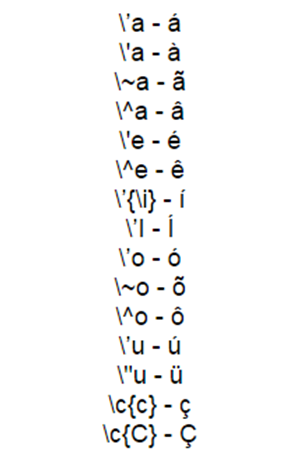
\includegraphics[scale=1.0]{USPSC-AcentuacaoLaTeX.png} \\
	Fonte: \citeonline{comandos}
	\end{center}	
\end{figure}

\chapter{Símbolos úteis em \LaTeX}
\begin{figure}[H]
	\begin{center}
		\caption{\label{fig_anexoc}Símbolos úteis em \LaTeX}
		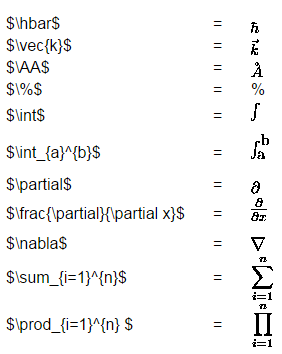
\includegraphics[scale=1.0]{USPSC-SimbolosUteis.png} \\
		Fonte: \citeonline{comandos}
	\end{center}	
\end{figure}


\chapter{Letras gregas em \LaTeX}
\begin{figure}[H]
	\begin{center}
		\caption{\label{fig_anexod}Letras gregas em \LaTeX}
		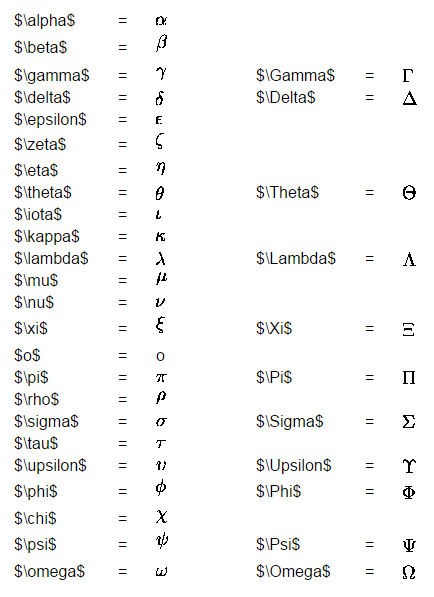
\includegraphics[scale=1.0]{USPSC-LetrasGregas.png} \\
		Fonte: \citeonline{comandos}
	\end{center}	
\end{figure}

\end{anexosenv}


%---------------------------------------------------------------------
% INDICE REMISSIVO
%--------------------------------------------------------------------
%% USPSC-IndicexRemissivos.tex
% ---
% Inicia os Índices Remissivos
% ---
%---------------------------------------------------------------------
% INDICE REMISSIVO
%--------------------------------------------------------------------
\phantompart
\printindex
%---------------------------------------------------------------------


%---------------------------------------------------------------------

\end{document}
